\documentclass[11pt]{report}

\usepackage[margin=1in]{geometry}
\usepackage[T1]{fontenc}
\usepackage{lmodern}
\usepackage{amsmath,amssymb}
\usepackage{graphicx}
\usepackage{booktabs}
\usepackage{array}
\usepackage{xcolor}
\usepackage{hyperref}
\usepackage{caption}
\usepackage{subcaption}
\usepackage{enumitem}
\usepackage{listings}
\usepackage{microtype}
\usepackage{float}
\usepackage{fancyhdr}
\usepackage{tikz}
\usetikzlibrary{arrows.meta,positioning,calc}

\hypersetup{
  colorlinks=true,
  linkcolor=blue!45!black,
  citecolor=blue!45!black,
  urlcolor=blue!45!black
}

\graphicspath{{figures/}}

\pagestyle{fancy}
\fancyhf{}
\fancyhead[L]{\small Assignment 1}
\fancyhead[R]{\small\leftmark}
\fancyfoot[C]{\thepage}
\renewcommand{\headrulewidth}{0.4pt}

\lstset{
  basicstyle=\ttfamily\small,
  breaklines=true,
  frame=single,
  backgroundcolor=\color{gray!5},
  showstringspaces=false,
  columns=fullflexible,
  keepspaces=true
}

\newcommand{\bx}{\mathbf{x}}
\newcommand{\bq}{\mathbf{q}}
\newcommand{\bu}{\mathbf{u}}
\newcommand{\bA}{\mathbf{A}}
\newcommand{\bB}{\mathbf{B}}
\newcommand{\bQ}{\mathbf{Q}}
\newcommand{\bR}{\mathbf{R}}

\title{\textbf{Assignment 1}\\[6pt]
Underactuated Robotics and Manipulation\\[4pt]
\large Acrobots, Cart-Poles, Quadrotors, Walking Models,\\
Legged Robots, and an Introduction to Manipulation}
\author{Zihao Liu\\[2pt]
Student ID: 220261979\\[2pt]
\texttt{213222647@seu.edu.cn}}
\date{October 2026}

\begin{document}
\maketitle

\begin{abstract}
This report documents the four parts of Assignment~1: three chapters of
\emph{Underactuated Robotics} (acrobots, cart-poles and quadrotors; simple
models of walking and running; highly-articulated legged robots) and the
introduction of \emph{Robotic Manipulation}.  I ran the supplied notebooks,
reproduced their main results, and added parameter and robustness studies
where they were useful.  The visible autograders pass: 13/13 and 12/12 for the
cart-pole notebooks, 13/13 for the hopper, 16/16 for the two footstep
planners, and 70/70, 50/50 and 50/50 for the manipulation exercises.  The
report gives the steps behind these numbers, the plots that show the behaviour,
and the code that produced them.  The less obvious cases---saturation,
non-minimum-phase zeros, the narrow compass-gait basin, and the partial
stability of the SLIP apex map---are discussed with the numerical evidence
rather than only stated as conclusions.
\end{abstract}

\tableofcontents

%=====================================================================
\chapter{Introduction}
%=====================================================================

\section{Scope of the assignment}

Assignment~1 covers four textbook chapters.  The first three belong to
\emph{Underactuated Robotics}; the last one is the introduction of
\emph{Robotic Manipulation}.  The required examples and exercise sections are
summarised in Table~\ref{tab:scope}.

\begin{table}[htbp]
\centering
\caption{Assignment~1 scope.}
\label{tab:scope}
\begin{tabular}{>{\raggedright\arraybackslash}p{0.20\textwidth}>{\raggedright\arraybackslash}p{0.38\textwidth}>{\raggedright\arraybackslash}p{0.30\textwidth}}
\toprule
Textbook chapter & Examples & Exercise section \\
\midrule
Ch.~3 Acrobots, Cart-Poles, and Quadrotors &
3.1, 3.2, 3.5, 3.6 & Section 3.8, Exercises 3.1--3.4 \\
Ch.~4 Simple Models of Walking and Running &
4.3, 4.4, 4.5, 4.6 & Section 4.6, one-dimensional hopper \\
Ch.~5 Highly-articulated Legged Robots &
5.1, 5.2 & Section 5.8, three exercises \\
Ch.~1 Introduction (Manipulation) &
1.2, 1.3 & Section 1.7, Exercises 1.1--1.4 \\
\bottomrule
\end{tabular}
\end{table}

\begin{table}[htbp]
\centering
\small
\caption{Coverage of the assignment items and where the corresponding code and
results can be found.}
\setlength{\tabcolsep}{4pt}\begin{tabular}{>{\raggedright\arraybackslash}p{0.20\textwidth}>{\raggedright\arraybackslash}p{0.11\textwidth}>{\raggedright\arraybackslash}p{0.38\textwidth}>{\raggedright\arraybackslash}p{0.20\textwidth}}
\toprule
Assignment item & Section & Code / notebook & Main result \\
\midrule
Example 3.1 & \S2.1 & \texttt{exp1\_analysis.py}, \texttt{Exp3'1-acrobot.ipynb} & 98\% / 63\% \\
Example 3.2 & \S2.2 & \texttt{cp\_analysis.py}, \texttt{Exp3'2-cartpole.ipynb} & 100\% / 36\% \\
Example 3.5 & \S2.3 & \texttt{lqr\_comparison.py} & conditions, zeros, LQR \\
Example 3.6 & \S2.4 & \texttt{quadrotor\_analysis.py} & settles in 1.08 s \\
Section 3.8 & \S2.5 & \texttt{cartpole\_balancing.ipynb}, \texttt{cartpoles\_urdf.ipynb} & 13/13, 12/12 \\
Example 4.3 & \S3.1 & \texttt{rimless\_wheel\_analysis.py} & fixed point \(\omega^\star\) \\
Example 4.4 & \S3.2 & \texttt{compass\_gait\_analysis.py} & 14 steps / 0.735 s \\
Examples 4.5--4.6 & \S3.3 & \texttt{slip\_analysis.py} & \(z^\star=0.8776\) m \\
Section 4.6 & \S3.4 & \texttt{one\_d\_hopper\_analysis.py} & 13/13 \\
Example 5.1 & \S4.1 & \texttt{zmp\_analysis.py} & 0.153 m \\
Example 5.2 & \S4.2 & \texttt{littledog\_analysis.py} & 0.6875 s stride \\
Section 5.8 & \S4.3 & \texttt{footstep\_analysis.py} & MIQP/GCS 16/16 \\
Example 1.2 & \S5.1 & teleoperation notebook & 3D demo ran \\
Example 1.3 & \S5.2 & this report & block diagrams \\
Section 1.7 & \S5.3 & four notebooks & 70/50/50 \\
\bottomrule
\end{tabular}
\end{table}

The examples are the supplied demonstrations: the code is already written and
the task is to run it, explain what is observed, and, where possible, study the
effect of changing a parameter.  The exercise sections are solved from scratch;
the report includes the derivations, the important code, and the relevant
plots.

\section{Environment and code}

All computations use Drake~1.58.0, the \texttt{underactuated} package
2026.9.8, and the \texttt{manipulation} package 2026.10.17 in the Python
environment \texttt{/Users/leo/venvs/drake/bin/python}.  The notebooks were
executed headlessly with \texttt{COLAB\_TESTING=1}; this prevents the MeshCat
visualizer from blocking on a browser connection.  The pinned
\texttt{drake\_models} package is used for the IIWA14, the WSG gripper and the
YCB object in the manipulation chapter.

The complete code accompanies the report as \texttt{Assignment\_1\_Code.zip}.
The files are listed in Appendix~\ref{app:code}.  For the reader who
wants to reproduce a specific result, the appendix gives the exact commands.

\section{Summary of results}

Table~\ref{tab:results} collects the automatic grading results.  They are
useful as a compact check that the code matches the expected behaviour; the
discussion in the following chapters explains what the numbers mean.

\begin{table}[htbp]
\centering
\caption{Automatic grading results.}
\label{tab:results}
\begin{tabular}{llc}
\toprule
Chapter & Item & Result \\
\midrule
Ch.~3 & \texttt{cartpole\_balancing.ipynb} & 13/13 \\
Ch.~3 & \texttt{cartpoles\_urdf.ipynb} & 12/12 \\
Ch.~4 & \texttt{one\_d\_hopper.ipynb} & 13/13 \\
Ch.~5 & MIQP footstep planning & 16/16 \\
Ch.~5 & GCS footstep planning & 16/16 \\
Ch.~1 & Drake Systems Fundamentals & 70/70 \\
Ch.~1 & Physics Simulation and Robot Loading & 50/50 \\
Ch.~1 & HardwareStation and Advanced Scenarios & 50/50 \\
\bottomrule
\end{tabular}
\end{table}

%=====================================================================
\part{Underactuated Systems}
%=====================================================================

%=====================================================================
\chapter{Acrobots, Cart-Poles, and Quadrotors}
%=====================================================================

\section{Example 3.1: Dynamics of the Acrobot}

The acrobot is a two-link planar robot whose shoulder is passive and whose
elbow is driven by a torque $u=\tau$ \cite{tedrake-acrobot}.  With
$q=[\theta_1,\theta_2]^\top$ and
$\bx=[\theta_1,\theta_2,\dot\theta_1,\dot\theta_2]^\top$, the manipulator
equations are
\[
M(q)\ddot q+C(q,\dot q)\dot q+G(q)=\begin{bmatrix}0\\ u\end{bmatrix}.
\]
The upright equilibrium is $\bx^\star=[\pi,0,0,0]^\top$.  At this point the
linearisation obtained in the notebook is
\[
\bA=\begin{bmatrix}
0&0&1&0\\
0&0&0&1\\
12.629&-12.693&-0.172&0.3015\\
-14.749&29.612&0.3015&-0.6033
\end{bmatrix},\qquad
\bB=\begin{bmatrix}0\\0\\-3.0147\\6.0332\end{bmatrix},
\]
with open-loop eigenvalues
$\{-6.492,-2.249,+2.231,+5.734\}$.  Two positive eigenvalues confirm that the
upright position is unstable.  The controllability matrix
$\mathcal C=[\bB,\bA\bB,\bA^2\bB,\bA^3\bB]$ has rank four, so the linearised
system is controllable even though the robot is underactuated.  The singular
values of $\mathcal C$ are $[511.7,123.1,0.0807,0.0715]$; the ratio between
the largest and the smallest is about $7\times10^3$, which indicates that some
directions are only weakly controllable.  The rank is four, but the smallest singular value is only
\(1.4	imes10^{-4}\) of the largest.  In the simulation this appeared as a
large initial elbow motion; the shoulder moved only after the elbow had built
up momentum.

With $Q=\operatorname{diag}(10,10,1,1)$ and $R=1$, the LQR gain is
\[
D=[\,278.44,\;112.29,\;119.72,\;56.83\,],\qquad u=D(\bx-\bx^\star),
\]
and the closed-loop poles are
$-10.126$, $-4.238$ and $-2.242\pm0.039j$.  A 100-trial study with initial
state $\bx_0=\bx^\star+0.05\,\mathcal N(0,I_4)$ gives a 98\% success rate
without saturation and 63\% with the $\pm10$~N\,m actuator limit.  The
successful trajectories show a pronounced non-minimum-phase undershoot: the
elbow first moves away from the target before the whole robot returns.

\begin{figure}[htbp]
\centering
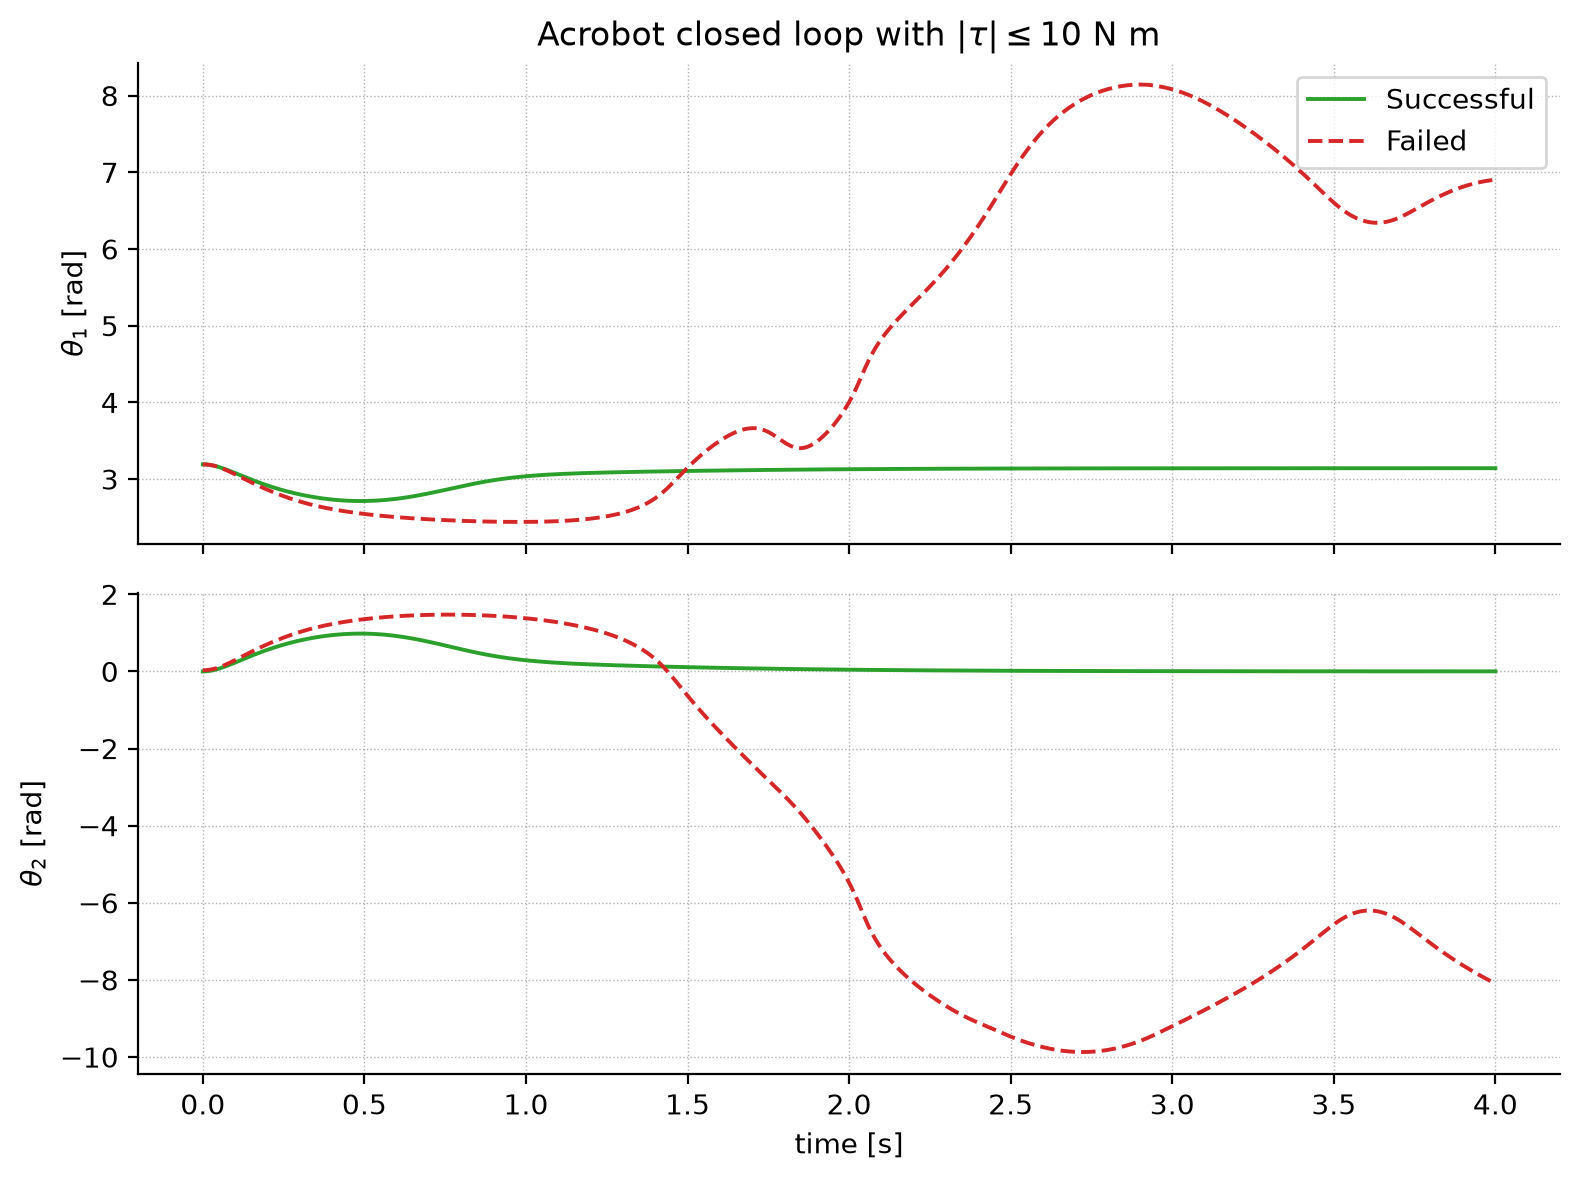
\includegraphics[width=0.78\textwidth]{ch3_acrobot_success.png}
\caption{Acrobot with the $\pm10$~N\,m saturation.  The green run starts with a
0.05~rad shoulder error; the red run also has a 0.03~rad elbow error and
saturates.  The elbow moves away from zero before the shoulder returns, which
is the non-minimum-phase undershoot.}
\end{figure}

Two parameters are especially important.  Increasing the distal mass $m_2$
from 0.5 to 4~kg reduces the minimum controllability singular value by a
factor of about 35 and the success rate from 98\% to 10\%; the peak torque
grows from 5~N\,m to more than 300~N\,m.  Changing $R$ from 1 to 100 reduces
the peak torque only from 11.2 to 9.7~N\,m, because the unstable open-loop
poles impose a finite gain even in the expensive-control limit.  In practice,
the acrobot needs a swing-up phase to enter the LQR region, and the actuator
limit must be included in the assessment.

\section{Example 3.2: Dynamics of the Cart-Pole}

The cart-pole has state $\bx=[x,\theta,\dot x,\dot\theta]^\top$ and input
$u=F_x$.  For the model used in the notebook, $m_c=10$~kg, $m_p=1$~kg and
$l_c=0.5$~m, the linearisation at $\bx^\star=[0,\pi,0,0]^\top$ is
\[
\bA=\begin{bmatrix}
0&0&1&0\\0&0&0&1\\0&0.981&0&0\\0&21.582&0&0
\end{bmatrix},\qquad
\bB=\begin{bmatrix}0\\0\\0.1\\0.2\end{bmatrix}.
\]
The open-loop eigenvalues are $0,0,\pm4.6456$.  The two zero eigenvalues come
from the cart position, which behaves as an integrator; the pair
$\pm4.6456$ is the unstable pole.  The controllability matrix is full rank,
with singular values $[4.326,4.326,0.0907,0.0907]$.  The transfer function from
$u$ to $x$ has a right-half-plane zero at $+4.43$, so the cart must first move
in the opposite direction before it can bring the pole back.  This is the
same non-minimum-phase mechanism as in the acrobot, seen more clearly in the
cart position.

With $Q=\operatorname{diag}(10,10,1,1)$ and $R=1$,
\[
D=[\,3.1623,\;-254.3925,\;9.7692,\;-55.1774\,],
\]
and the closed-loop poles are $-4.7206$, $-4.5739$ and
$-0.3820\pm0.3761j$.  The two fast poles bring the pole back; the slow pair is
the cart returning to the origin.  The original notebook does not limit the
force, and a 100-trial study with $\bx_0=\bx^\star+0.1\,\mathcal N(0,I_4)$
balances the pole in 100\% of the trials.  The median peak force is about
17~N, with a 90th percentile near 40~N.  When the force is limited, the
picture changes: 20~N gives 90\% pole-balancing success, 5~N gives 36\%, and
2~N fails in most trials because the non-minimum-phase recovery needs a
larger control authority.

\begin{figure}[htbp]
\centering
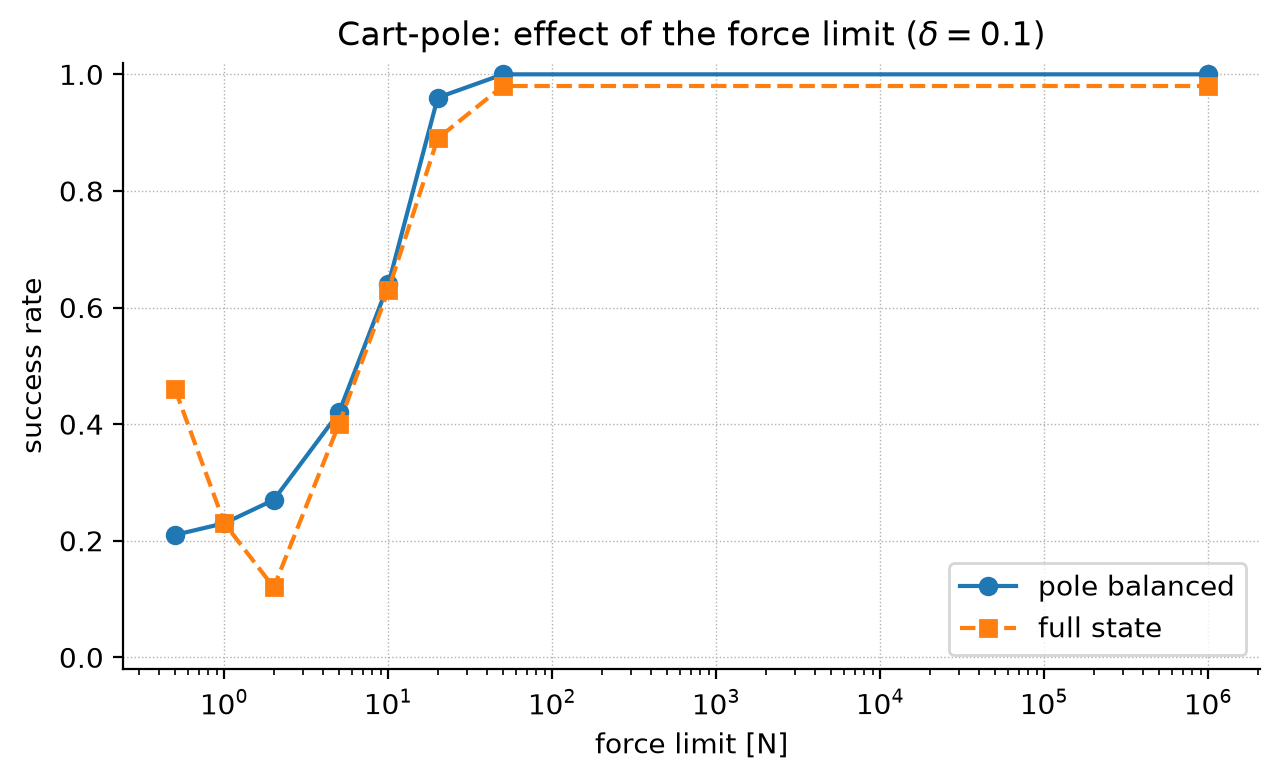
\includegraphics[width=0.72\textwidth]{ch3_cartpole_force.png}
\caption{Cart-pole success rate versus force limit at $\delta=0.1$.  At 20~N the
pole still balances in 90\% of trials; at 10~N the rate is 64\%, and at 5~N
only 36\%.  Without a limit the pole is easy; the actuator is the binding
constraint.}
\end{figure}

The cart mass is the most important physical parameter.  From 2 to 20~kg the
median peak force grows from about 5 to 32~N, and the full-state success rate
falls from 100\% to 68\%; the pole itself remains balanceable.  Increasing
$R$ saves force but slows the cart-return mode: for $R=100$ the slow pole is
about $-0.12$~rad/s, so a 5~s simulation is too short for the cart to return.

\section{Example 3.5: LQR for the Acrobot and Cart-Pole}

The acrobot and the cart-pole are useful together because they have the same
control structure but different modal properties.  Both are controllable and
both are non-minimum phase.  The acrobot's condition number is about 150 times
larger, which reflects the weaker coupling through the passive shoulder.  The
cart-pole has two zero eigenvalues and therefore a slow cart mode, while the
acrobot has four relatively fast modes.  These differences explain why the
same LQR weight has a different effect on the two systems: increasing $R$
mainly reduces the torque on the acrobot, but it substantially slows the cart
return on the cart-pole.

\begin{figure}[htbp]
\centering
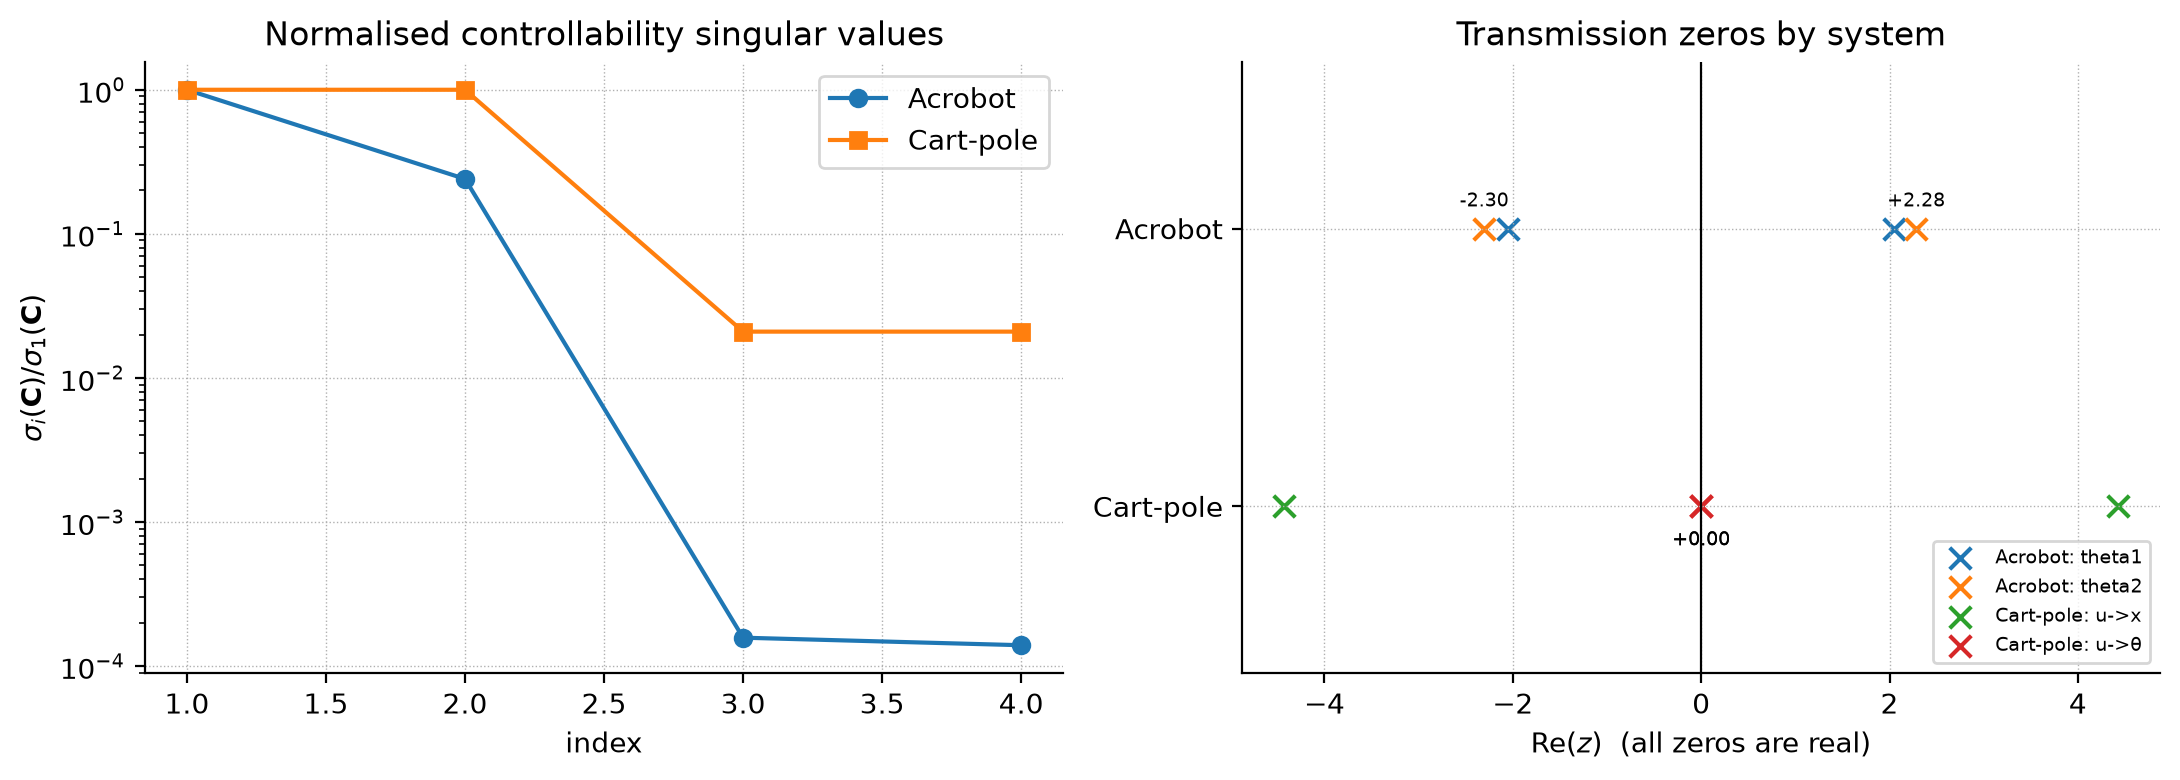
\includegraphics[width=0.88\textwidth]{ch3_lqr_linear.png}
\caption{Normalised controllability singular values and transmission zeros.
The acrobot's smallest normalized singular value is about
\(1.4\times10^{-4}\); the cart-pole's is about \(2.1\times10^{-2}\).  Both have
right-half-plane zeros: the acrobot at $+2.05$ and $+2.28$, the cart-pole at
$+4.43$.}
\end{figure}

\section{Example 3.6: LQR for Quadrotors}

The planar quadrotor has state
$\bx=[x,z,\theta,\dot x,\dot z,\dot\theta]^\top$ and two thrust inputs.  At
hover, $u_1+u_2=mg$ and $\theta=0$.  The textbook LQR uses
\[
\bQ=\operatorname{diag}\!\left(10,10,10,1,1,\frac{l}{2\pi}\right),
\qquad
\bR=\begin{bmatrix}0.1&0.05\\0.05&0.1\end{bmatrix}.
\]
The closed-loop poles are $-80.75$, $-15.86$, $-6.59$, $-3.60$ and
$-2.72\pm1.61j$.  From an initial tilt of 0.2~rad the controller settles in
about 0.06~s with a peak thrust of 5.17~N; ten random initial conditions with
standard deviation 0.1 all recover.

The sensitivity study shows the expected trade-offs.  Increasing the position
weight makes the response faster but raises the peak thrust.  Increasing $R$
reduces the peak thrust at the cost of a slower response.  A constant wind
produces a steady-state offset because LQR has no integral action: the offset
is about 0.073~m at 0.25~N and 0.554~m at 2~N.  The initial tilt is recovered
for all tested values up to 0.7~rad.

\begin{figure}[htbp]
\centering
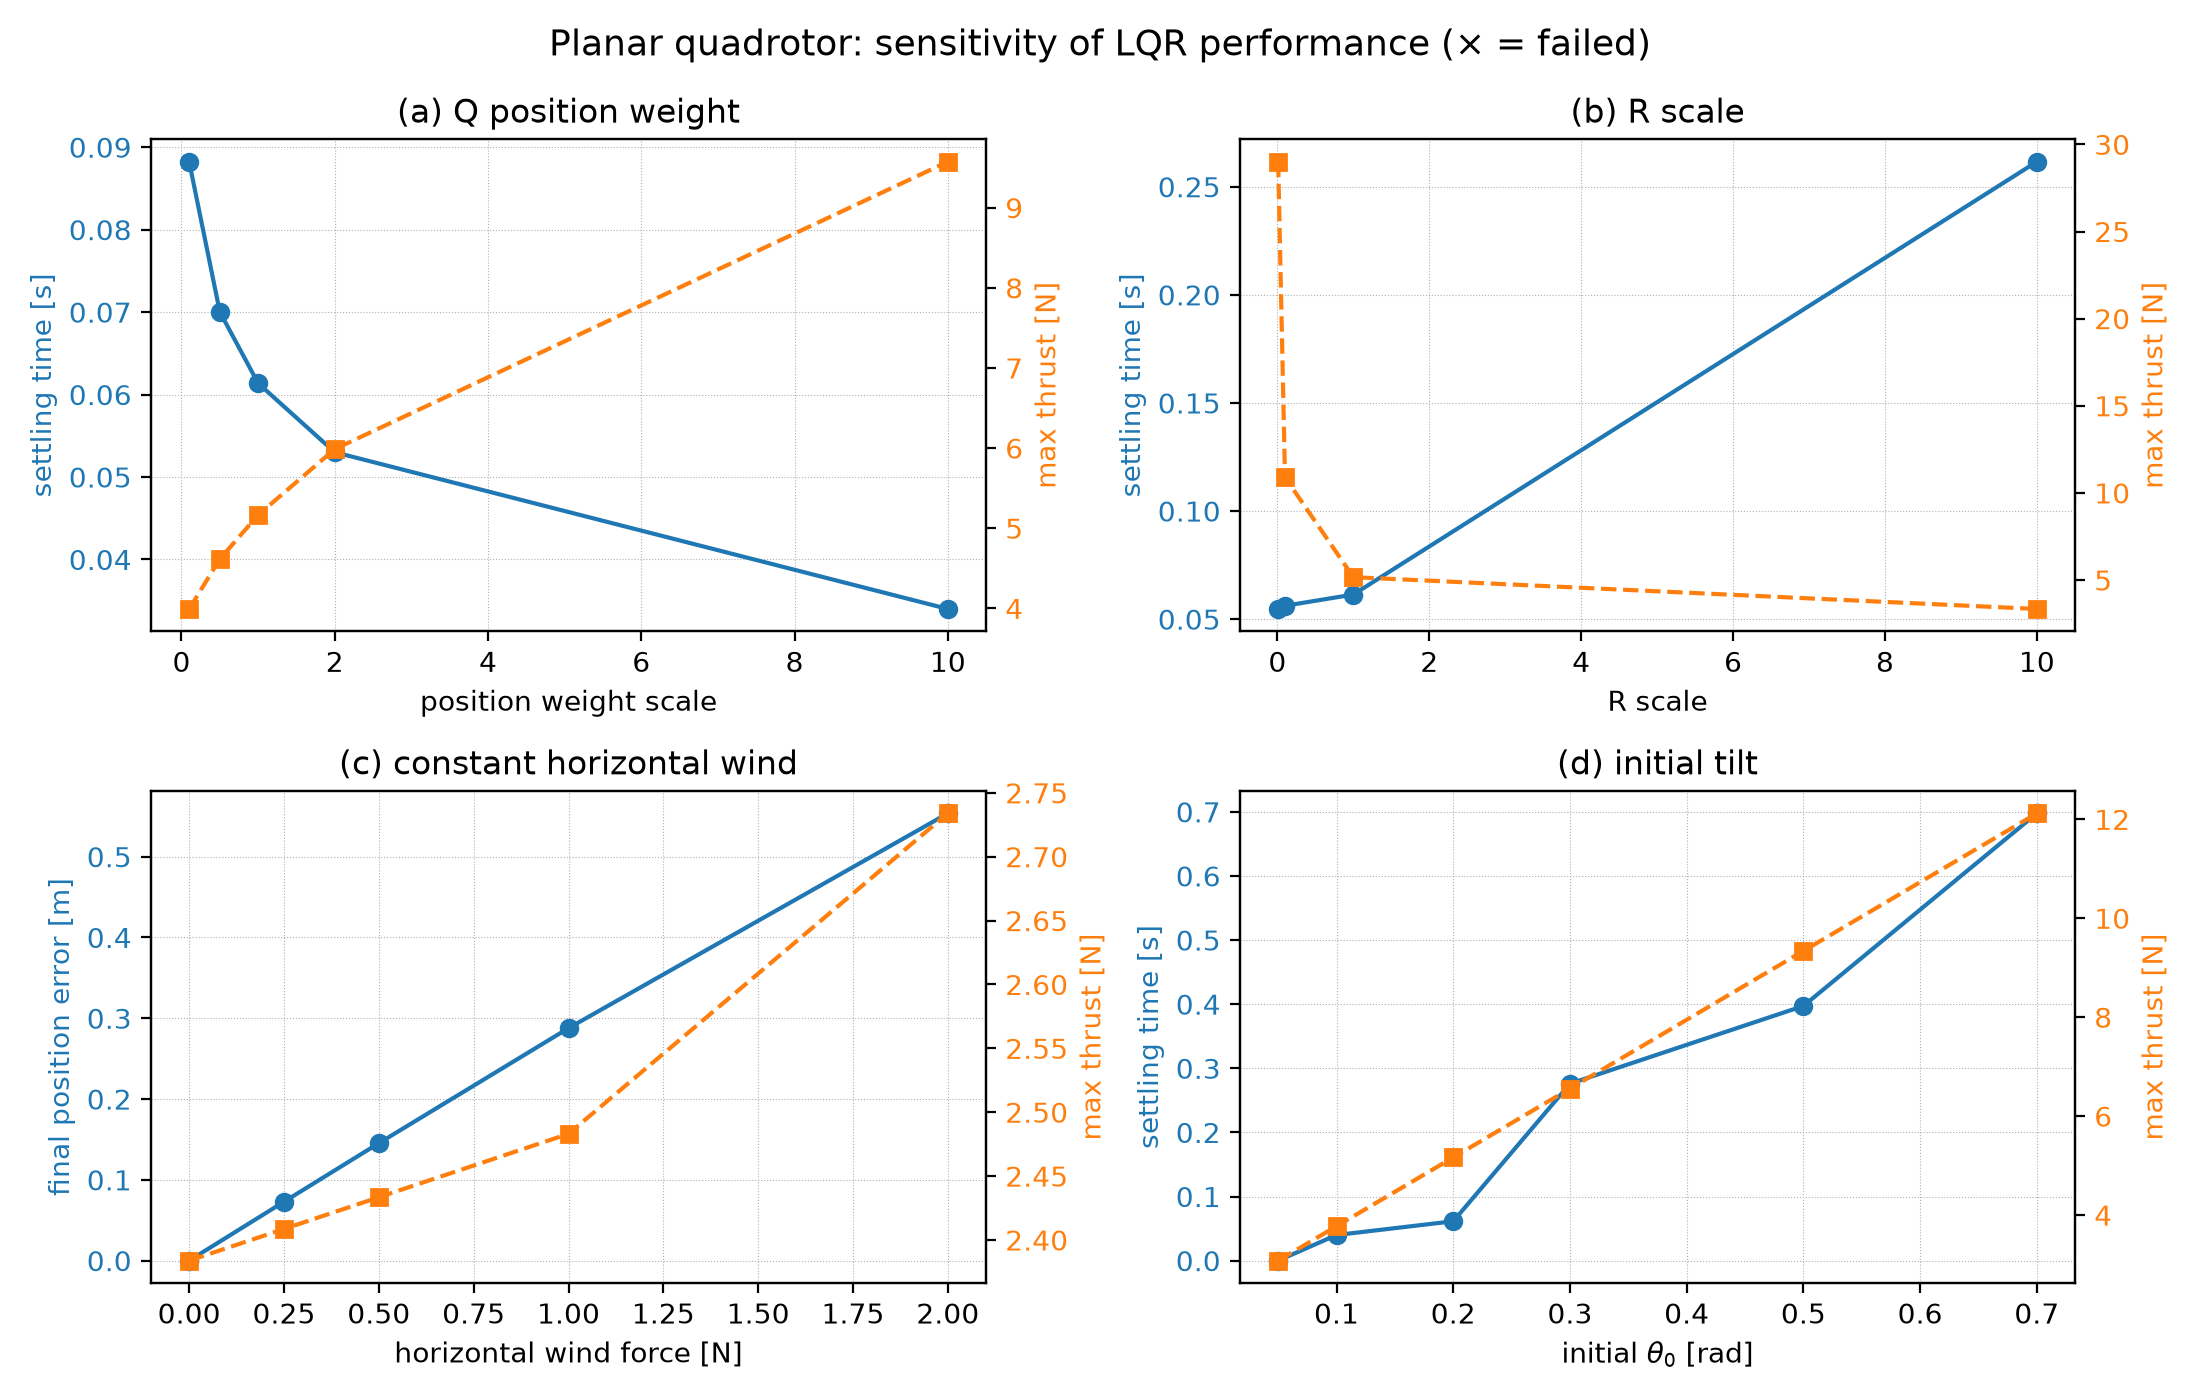
\includegraphics[width=0.95\textwidth]{ch3_quad_sensitivity.png}
\caption{Planar quadrotor sensitivity.  With 0.25~N wind the steady-state offset
is 0.073~m; with 2~N it is 0.554~m.  The other panels show the expected
$Q/R$ trade-off.}
\end{figure}

The 3D quadrotor has four thrust inputs and six degrees of freedom.  It is
underactuated, but the hover equilibrium is stabilisable.  The LQR is
linearised around a point where the total thrust balances gravity, not around
zero thrust.  From a 0.2~rad roll and 0.1~rad pitch perturbation the official
stabilising controller and our LQR both return to hover in about 1.08~s with a
peak thrust near 3~N.  The sensitivity to $Q$, $R$ and initial tilt follows
the same pattern as in the planar case.

\section{Section 3.8: Exercises 3.1--3.4}

\subsection{Exercise 3.1: linearisation and balancing}

For the cart-pole with $m_c=m_p=l=1$ and $g=9.81$, the equations used in the
notebook are
\[
\ddot x=\frac{u+\sin\theta(\dot\theta^2+g\cos\theta)}{1+\sin^2\theta},
\qquad
\ddot\theta=\frac{-u\cos\theta-\dot\theta^2\cos\theta\sin\theta-2g\sin\theta}
{1+\sin^2\theta}.
\]
At the upright point $\bx^\star=[0,\pi,0,0]^\top$,
\[
\bA_{\rm lin}=\begin{bmatrix}
0&0&1&0\\0&0&0&1\\0&9.81&0&0\\0&19.62&0&0
\end{bmatrix},\qquad
\bB_{\rm lin}=\begin{bmatrix}0\\0\\1\\1\end{bmatrix}.
\]
The linearisation error is small near the equilibrium and grows quickly with
distance.  At $\theta=0.99\pi$ the error is $9\times10^{-4}$; at
$\theta=\pi/2$ it is 26.05; at $\theta=0$ it is 68.91.  The error also depends
on the input when $\theta\neq\pi$, because the nonlinear input gains
$1/(1+\sin^2\theta)$ and $-\cos\theta/(1+\sin^2\theta)$ are replaced by
constants in the linear model.  The cart position $x$ does not appear in the
dynamics, so it does not affect the error.

With $Q=I_4$ and $R=1$, the LQR gain is
\[
K=[-1.0000,\;51.0612,\;-2.7221,\;12.8277],\qquad u=-K(\bx-\bx^\star),
\]
and the closed-loop poles are $-5.0417,-3.9438,-0.5600\pm0.4239j$.  The six
initial states from the notebook are simulated for 5~s; the controller
recovers from states 0, 1, 2 and 5:
\[
\texttt{system\_recovers\_from\_states}=[0,1,2,5].
\]
The first three are close to the upright point.  State 5 has $\theta=\pi$ and
only a cart offset, which is linearly controllable.  States 3
($\theta=\pi/2$) and 4 ($\theta=0$) lie outside the region where the
linearisation is useful; the controller fails there, as the error table
predicts.

\begin{figure}[htbp]
\centering
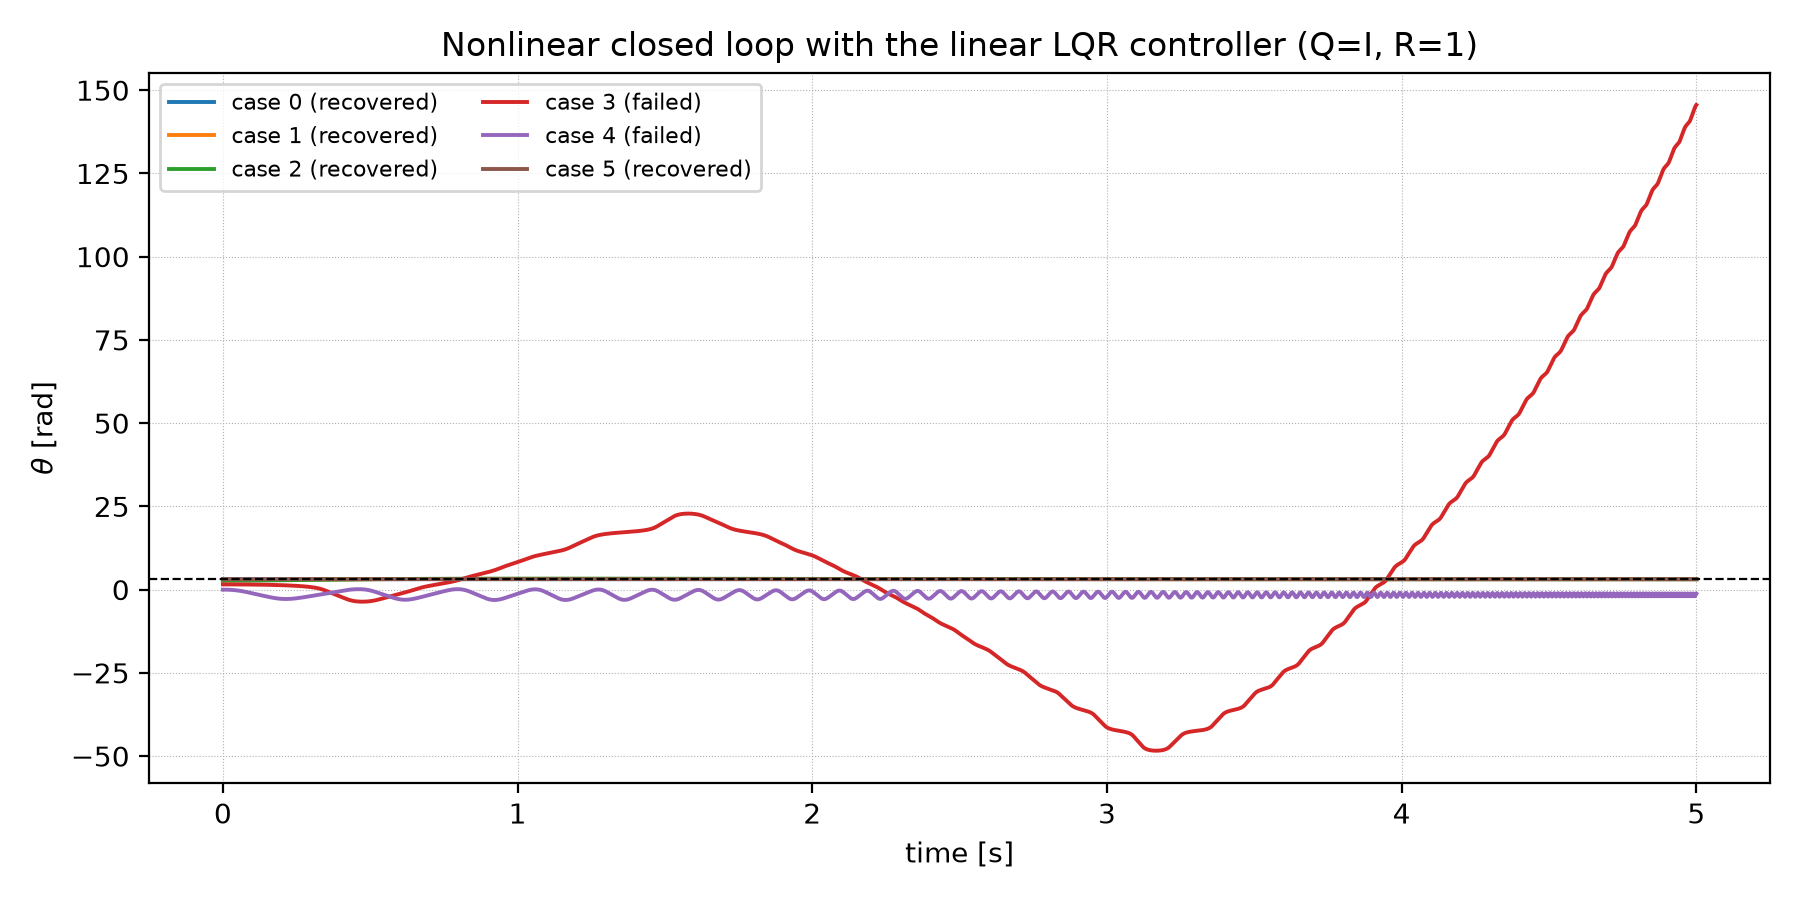
\includegraphics[width=0.8\textwidth]{ch3_cartpole_closed_loop.png}
\caption{Closed-loop angle histories for the six initial states of Exercise~3.1.
Cases 3 ($\theta=\pi/2$) and 4 ($\theta=0$) leave the upright region; the
linear controller was designed for the tangent at $\pi$.}
\end{figure}

\subsection{Exercise 3.2: cart-pole URDFs}

The single pendulum URDF has a base of mass 1 at the origin, a pendulum whose
ball of mass 1 is at $z=-1$, a spherical visual of radius 0.05 and a
cylindrical rod of length 1 and radius 0.01 centred at $z=-0.5$.  The joint
\texttt{theta0} connects the base to the pendulum, with origin $(0,0,0)$ and
axis $(0,-1,0)$.  The unstable equilibrium is $\bx^\star=[0,\pi,0,0]^\top$.

The double pendulum needs more care with the frames.  The second joint is at
the ball of the first pendulum, i.e.\ at $(0,0,-1)$ in the
\texttt{pendulum0} frame.  The second link has its ball at $z=+1$ in its own
frame.  With $\theta_1=0$ the second pendulum points back towards the cart and
overlaps the first; with $\theta_0=\theta_1=\pi$ both pendula stand upright.
The equilibrium is $\bx^\star=[0,\pi,\pi,0,0,0]^\top$.

The LQR is designed directly from the nonlinear \texttt{MultibodyPlant}.  For
the single pendulum with $Q=\operatorname{diag}(10,10,1,1)$ and $R=1$,
\[
K=[-3.1623,\;61.3987,\;-5.2854,\;16.1699],
\]
with poles $-4.8948,-4.0983,-0.9457\pm0.8075j$.  After 5~s the angle error is
0.0036~rad and the peak force is 19.3~N.  For the double pendulum with
$Q=\operatorname{diag}(10,10,10,1,1,1)$,
\[
K=[3.1623,\;-54.8416,\;-300.4370,\;7.4384,\;-54.0081,\;-68.9418],
\]
with poles
$-7.5798,-6.1385,-3.6749,-3.4281,-0.7754\pm0.6611j$.  The two angle errors
after 5~s are 0.0142 and 0.0007~rad, and the peak force is 66.6~N.  The
autograder gives 12/12.

\begin{figure}[htbp]
\centering
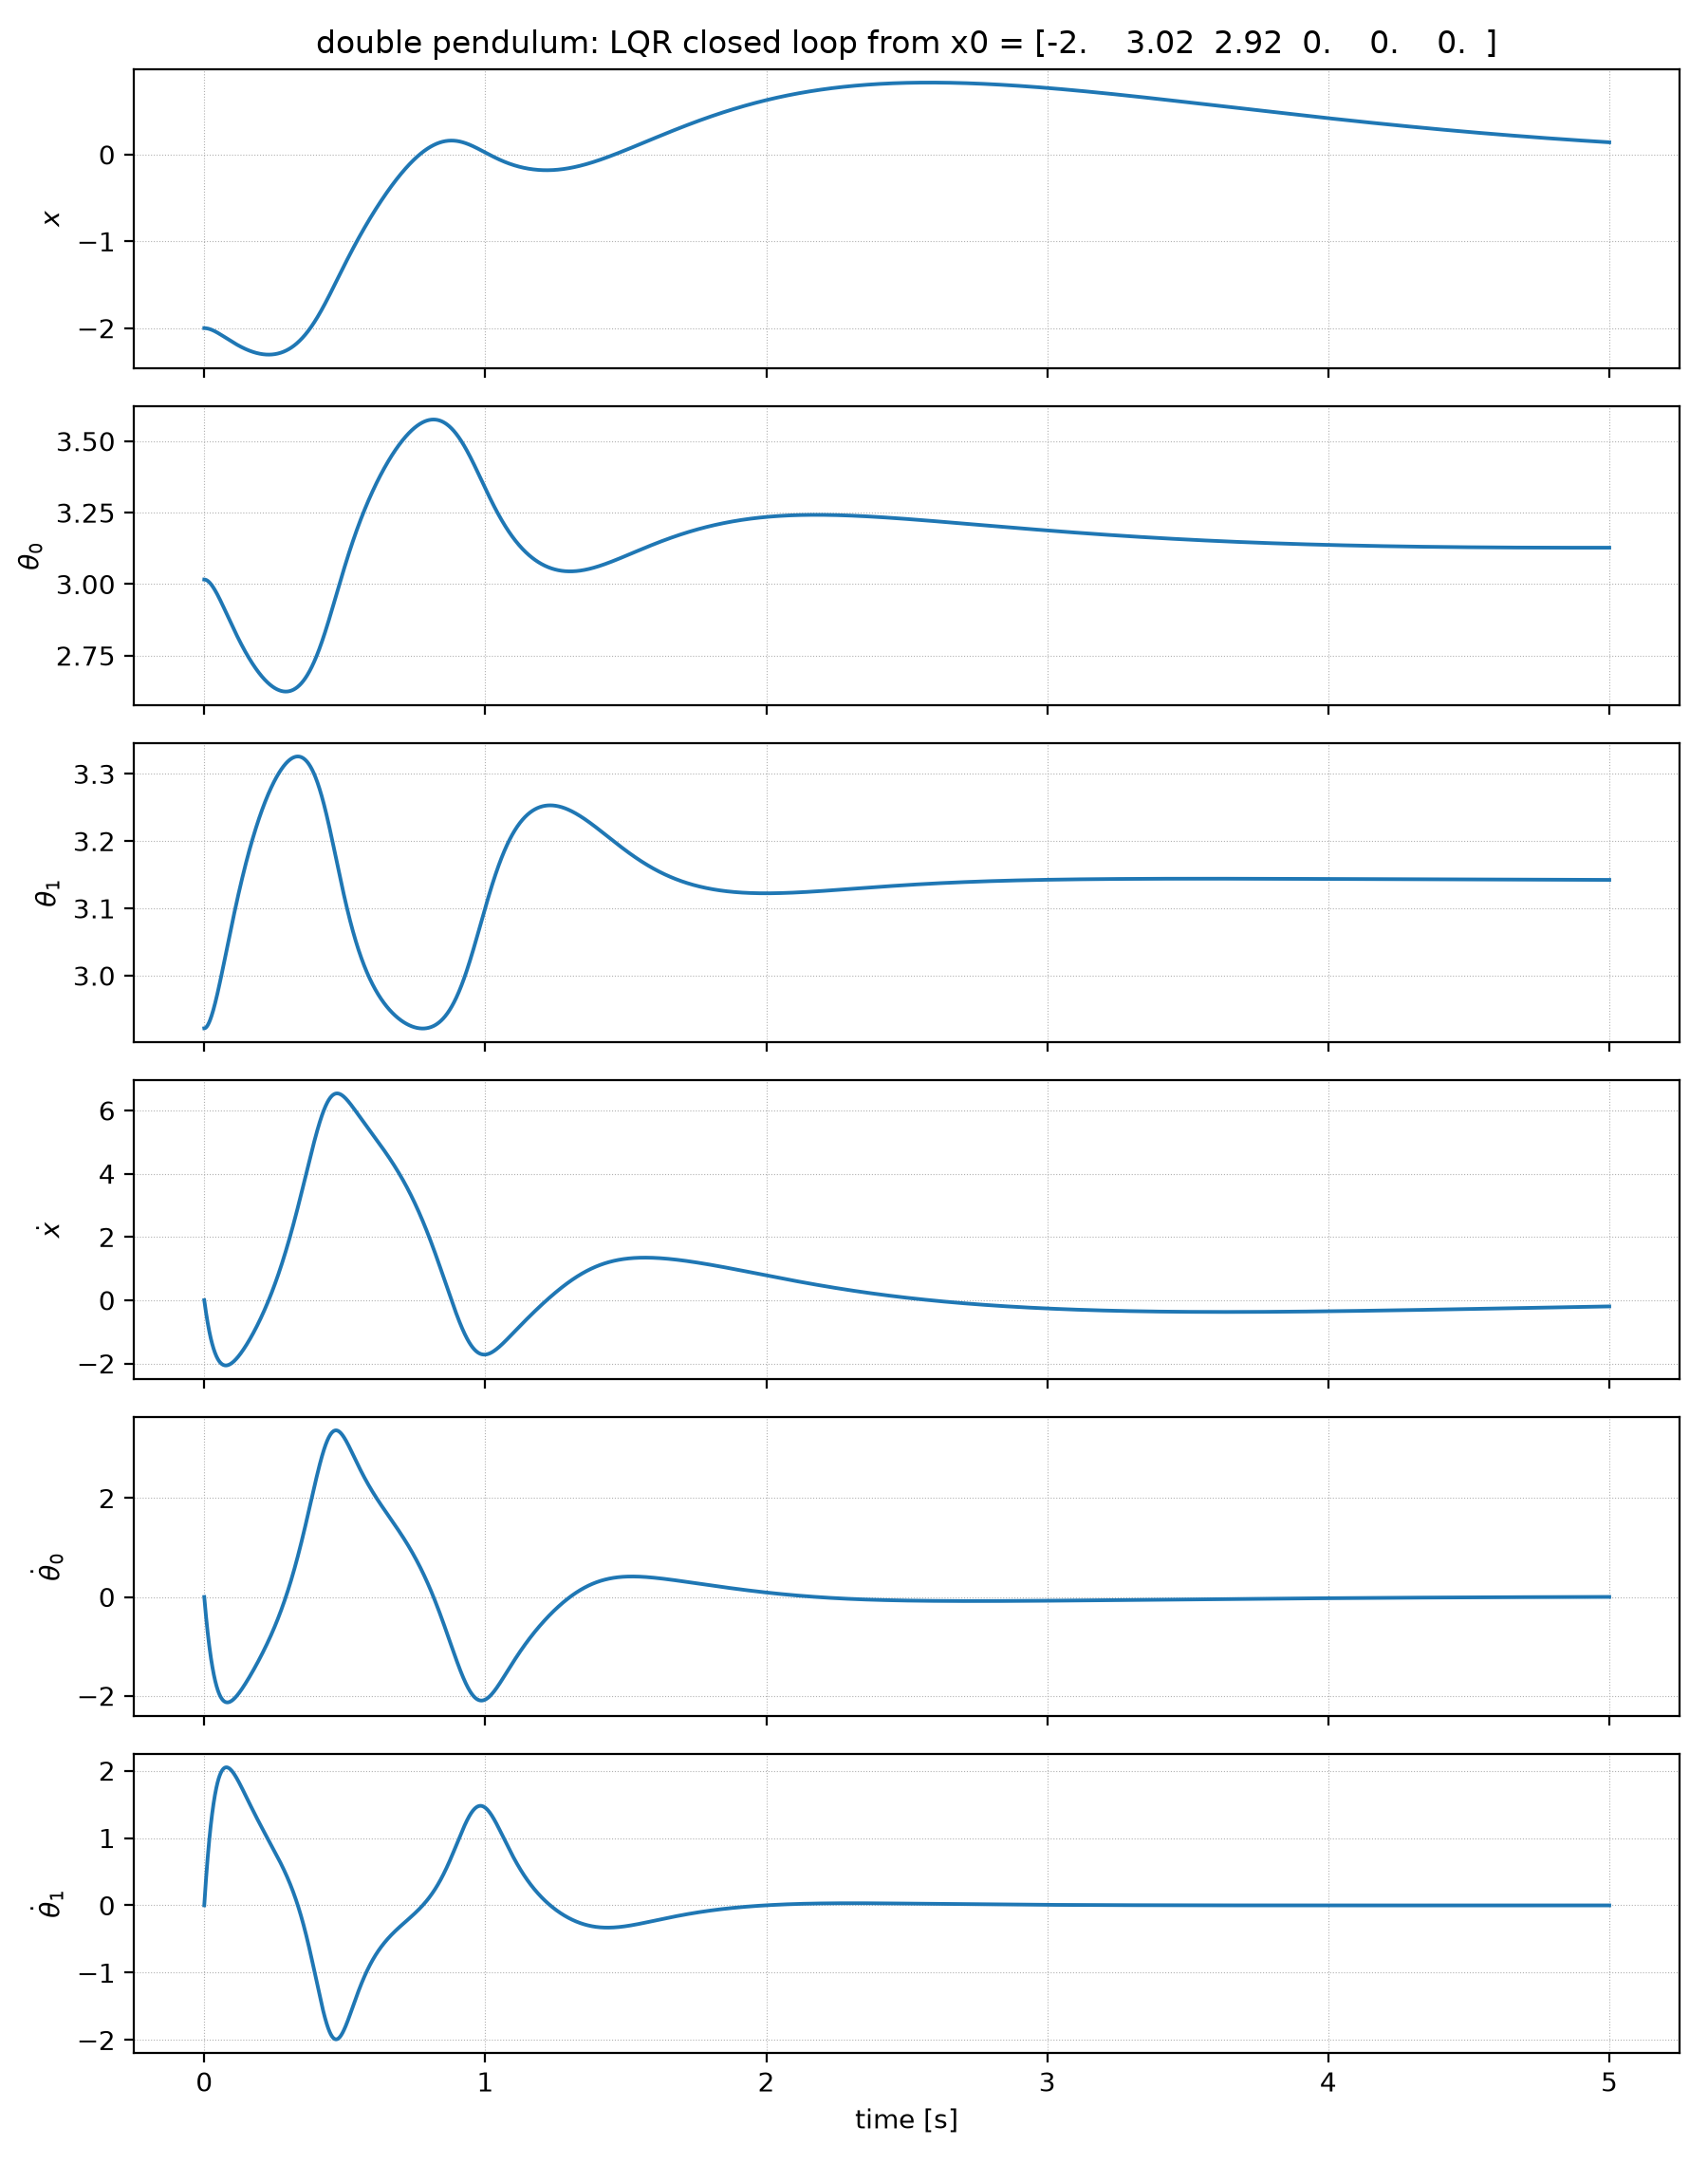
\includegraphics[width=0.9\textwidth]{ch3_double_balancing.png}
\caption{Double-pendulum cart-pole under LQR.  The angle errors at 5~s are 0.014
and 0.0007~rad, but the cart is still moving; the slow pair of poles has a
time constant of about 1.3~s.}
\end{figure}

\subsection{Exercise 3.3: controllability}

The discrete double integrator
\[
x_1[n+1]=x_1[n]+x_2[n],\qquad x_2[n+1]=x_2[n]+u[n],
\qquad x_1,x_2,u\in\mathbb Z
\]
maps $s_{i,j}$ to $(i+j,j+u)$.  Figure~\ref{fig:grid} shows the edges for
$u=-1,0,+1$.  From $s_{0,0}$, one step gives $(0,u_0)$, so $x_1=0$ and no
state with $i>0$ is reachable.  Two steps give $(u_0,u_0+u_1)$; choosing
$u_0=i$ and $u_1=j-i$ reaches any $s_{i,j}$.  For an arbitrary start
$s_{i_1,j_1}$ and goal $s_{i_2,j_2}$, the two-step controls are
\[
u_0=i_2-i_1-2j_1,\qquad
u_1=j_2+j_1+i_1-i_2.
\]
One step is not enough in general because it fixes $x_1[1]=i_1+j_1$.

\begin{figure}[htbp]
\centering
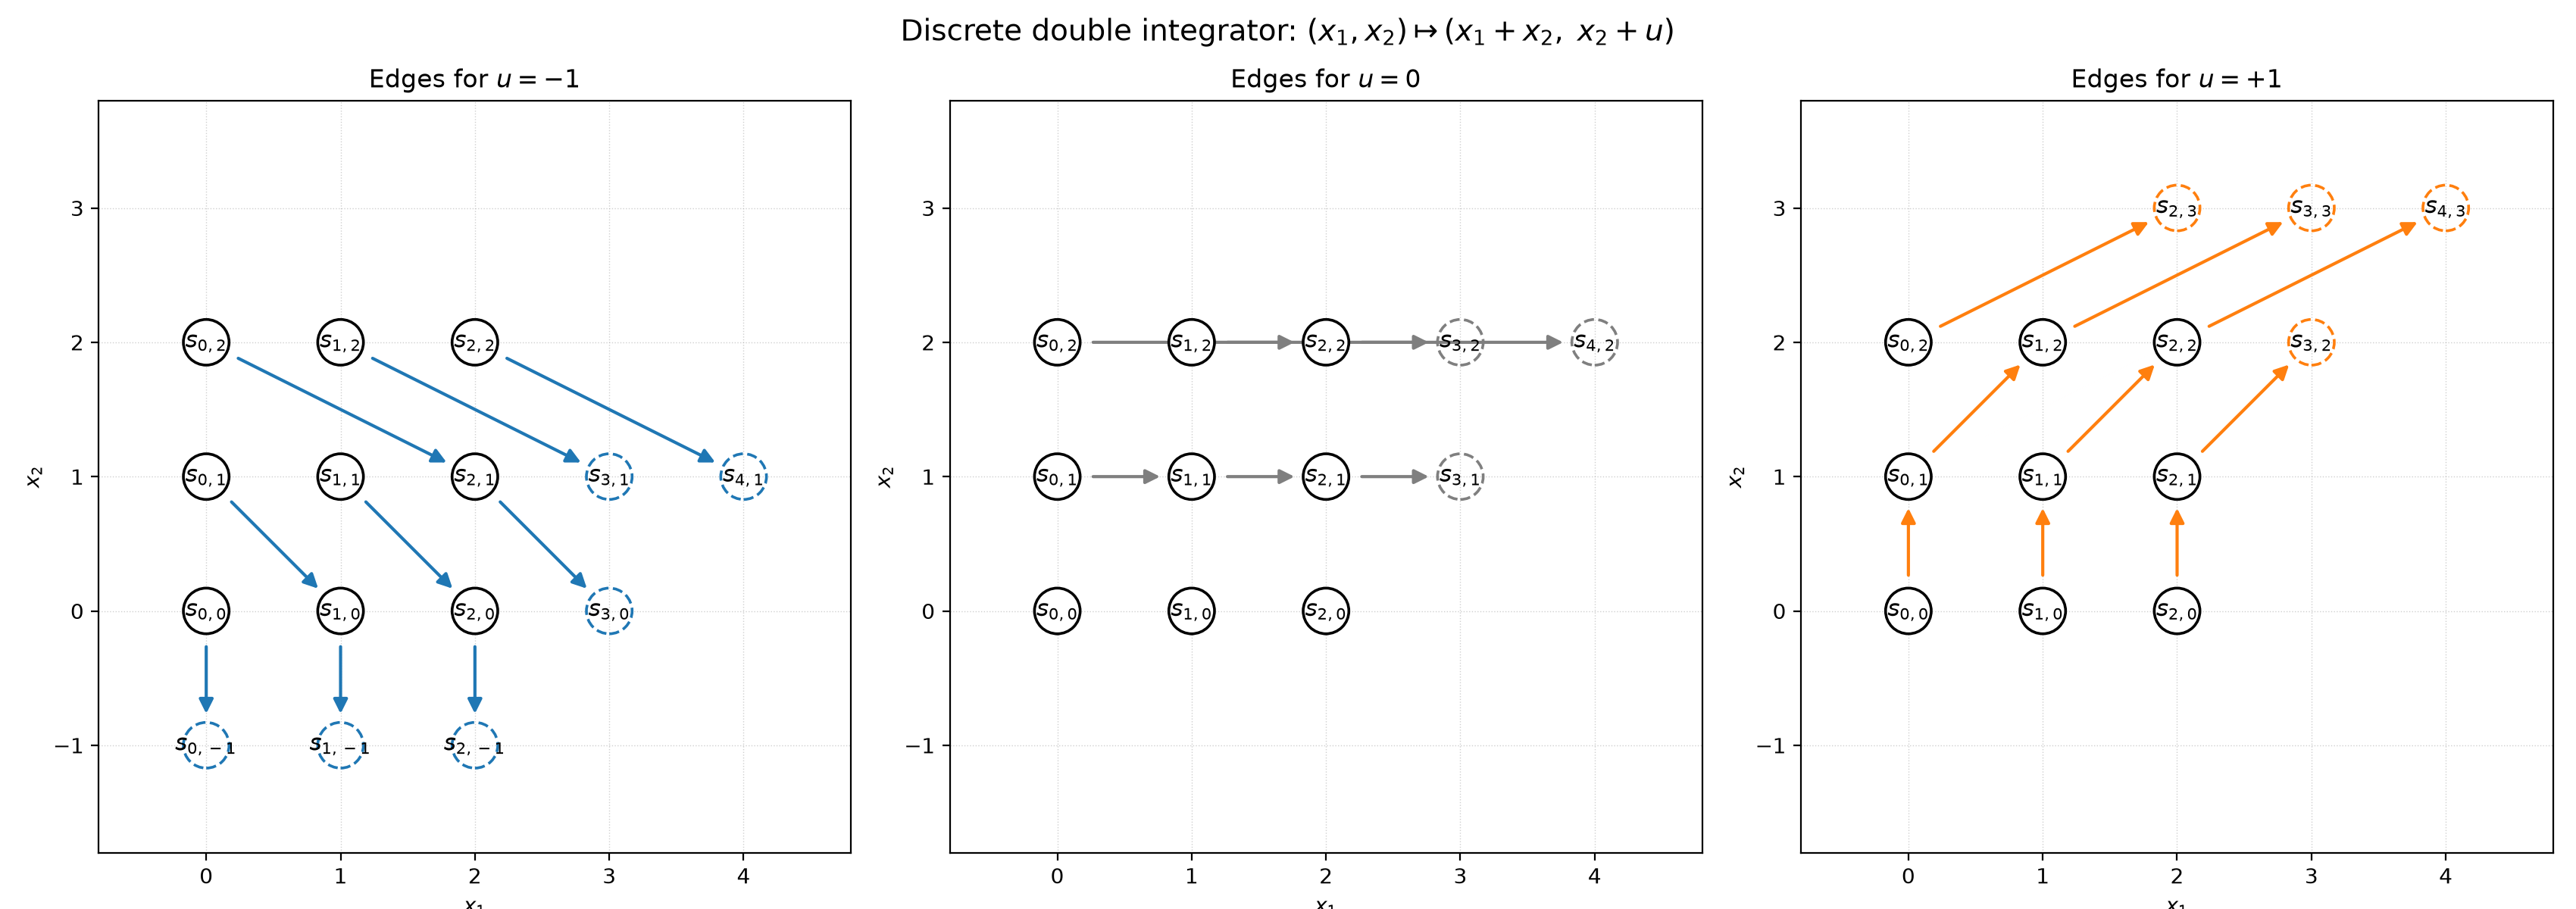
\includegraphics[width=0.95\textwidth]{ch3_grid.png}
\caption{Edges of the discrete double integrator for $u=-1,0,+1$.  The source
nodes are solid; destinations outside the $3\times3$ grid are dashed.  The
two-step construction $s_{0,0}\to(0,i)\to(i,j)$ is the path used in the text.}
\label{fig:grid}
\end{figure}

For continuous LTI systems, the four pairs are tested with the controllability
matrix.  $(\bA_1,\bB_1)$ and $(\bA_2,\bB_2)$ have rank one and are not
controllable: in the first, $x_1$ is decoupled from the input; in the second,
$z=x_1-x_2$ satisfies $\dot z=z$ independently of $u$.  $(\bA_3,\bB_3)$ and
$(\bA_4,\bB_4)$ are controllable.  For $(\bA_4,\bB_4)$ the controllability
matrix has rank four; the eigenvalues are $0,0,\pm\sqrt2$ and the PBH test is
full rank at each eigenvalue.  In the second-order interpretation,
$(\bA_3,\bB_3)$ is fully actuated (one degree of freedom, one input), while
$(\bA_4,\bB_4)$ is underactuated ($q=[x,\theta]$, only $x$ actuated).  This
again separates controllability from full actuation.

\subsection{Exercise 3.4: stability and linearisation}

For the pendulum with $m=l=1$ and damping $b$,
\[
\dot\theta=\omega,\qquad \dot\omega=-g\sin\theta-b\omega,
\]
the equilibrium points are $(0,0)$ and $(\pi,0)$, with Jacobian
\[
A(\theta^\star)=\begin{bmatrix}0&1\\-g\cos\theta^\star&-b\end{bmatrix}.
\]
The eigenvalues are $\pm3.1321j$ for $b=0$ at the bottom, $\pm3.1321$ for
$b=0$ at the top, $-0.5\pm3.0919j$ for $b=1$ at the bottom, and
$2.6718,-3.6718$ for $b=1$ at the top.

The stability table follows from these values and from the phase portraits.
At the undamped bottom the nonlinear system has closed orbits: it is stable
i.s.L.\ but not asymptotically or exponentially stable.  The linearisation is
a centre; when the real part is zero the linearisation theorem is
inconclusive, and the energy argument is needed.  At the top the saddle
structure makes both the nonlinear system and its linearisation unstable.
With damping, the bottom becomes locally exponentially stable; the top still
has one positive eigenvalue, so damping alone cannot stabilise the inverted
pendulum.

\begin{figure}[htbp]
\centering
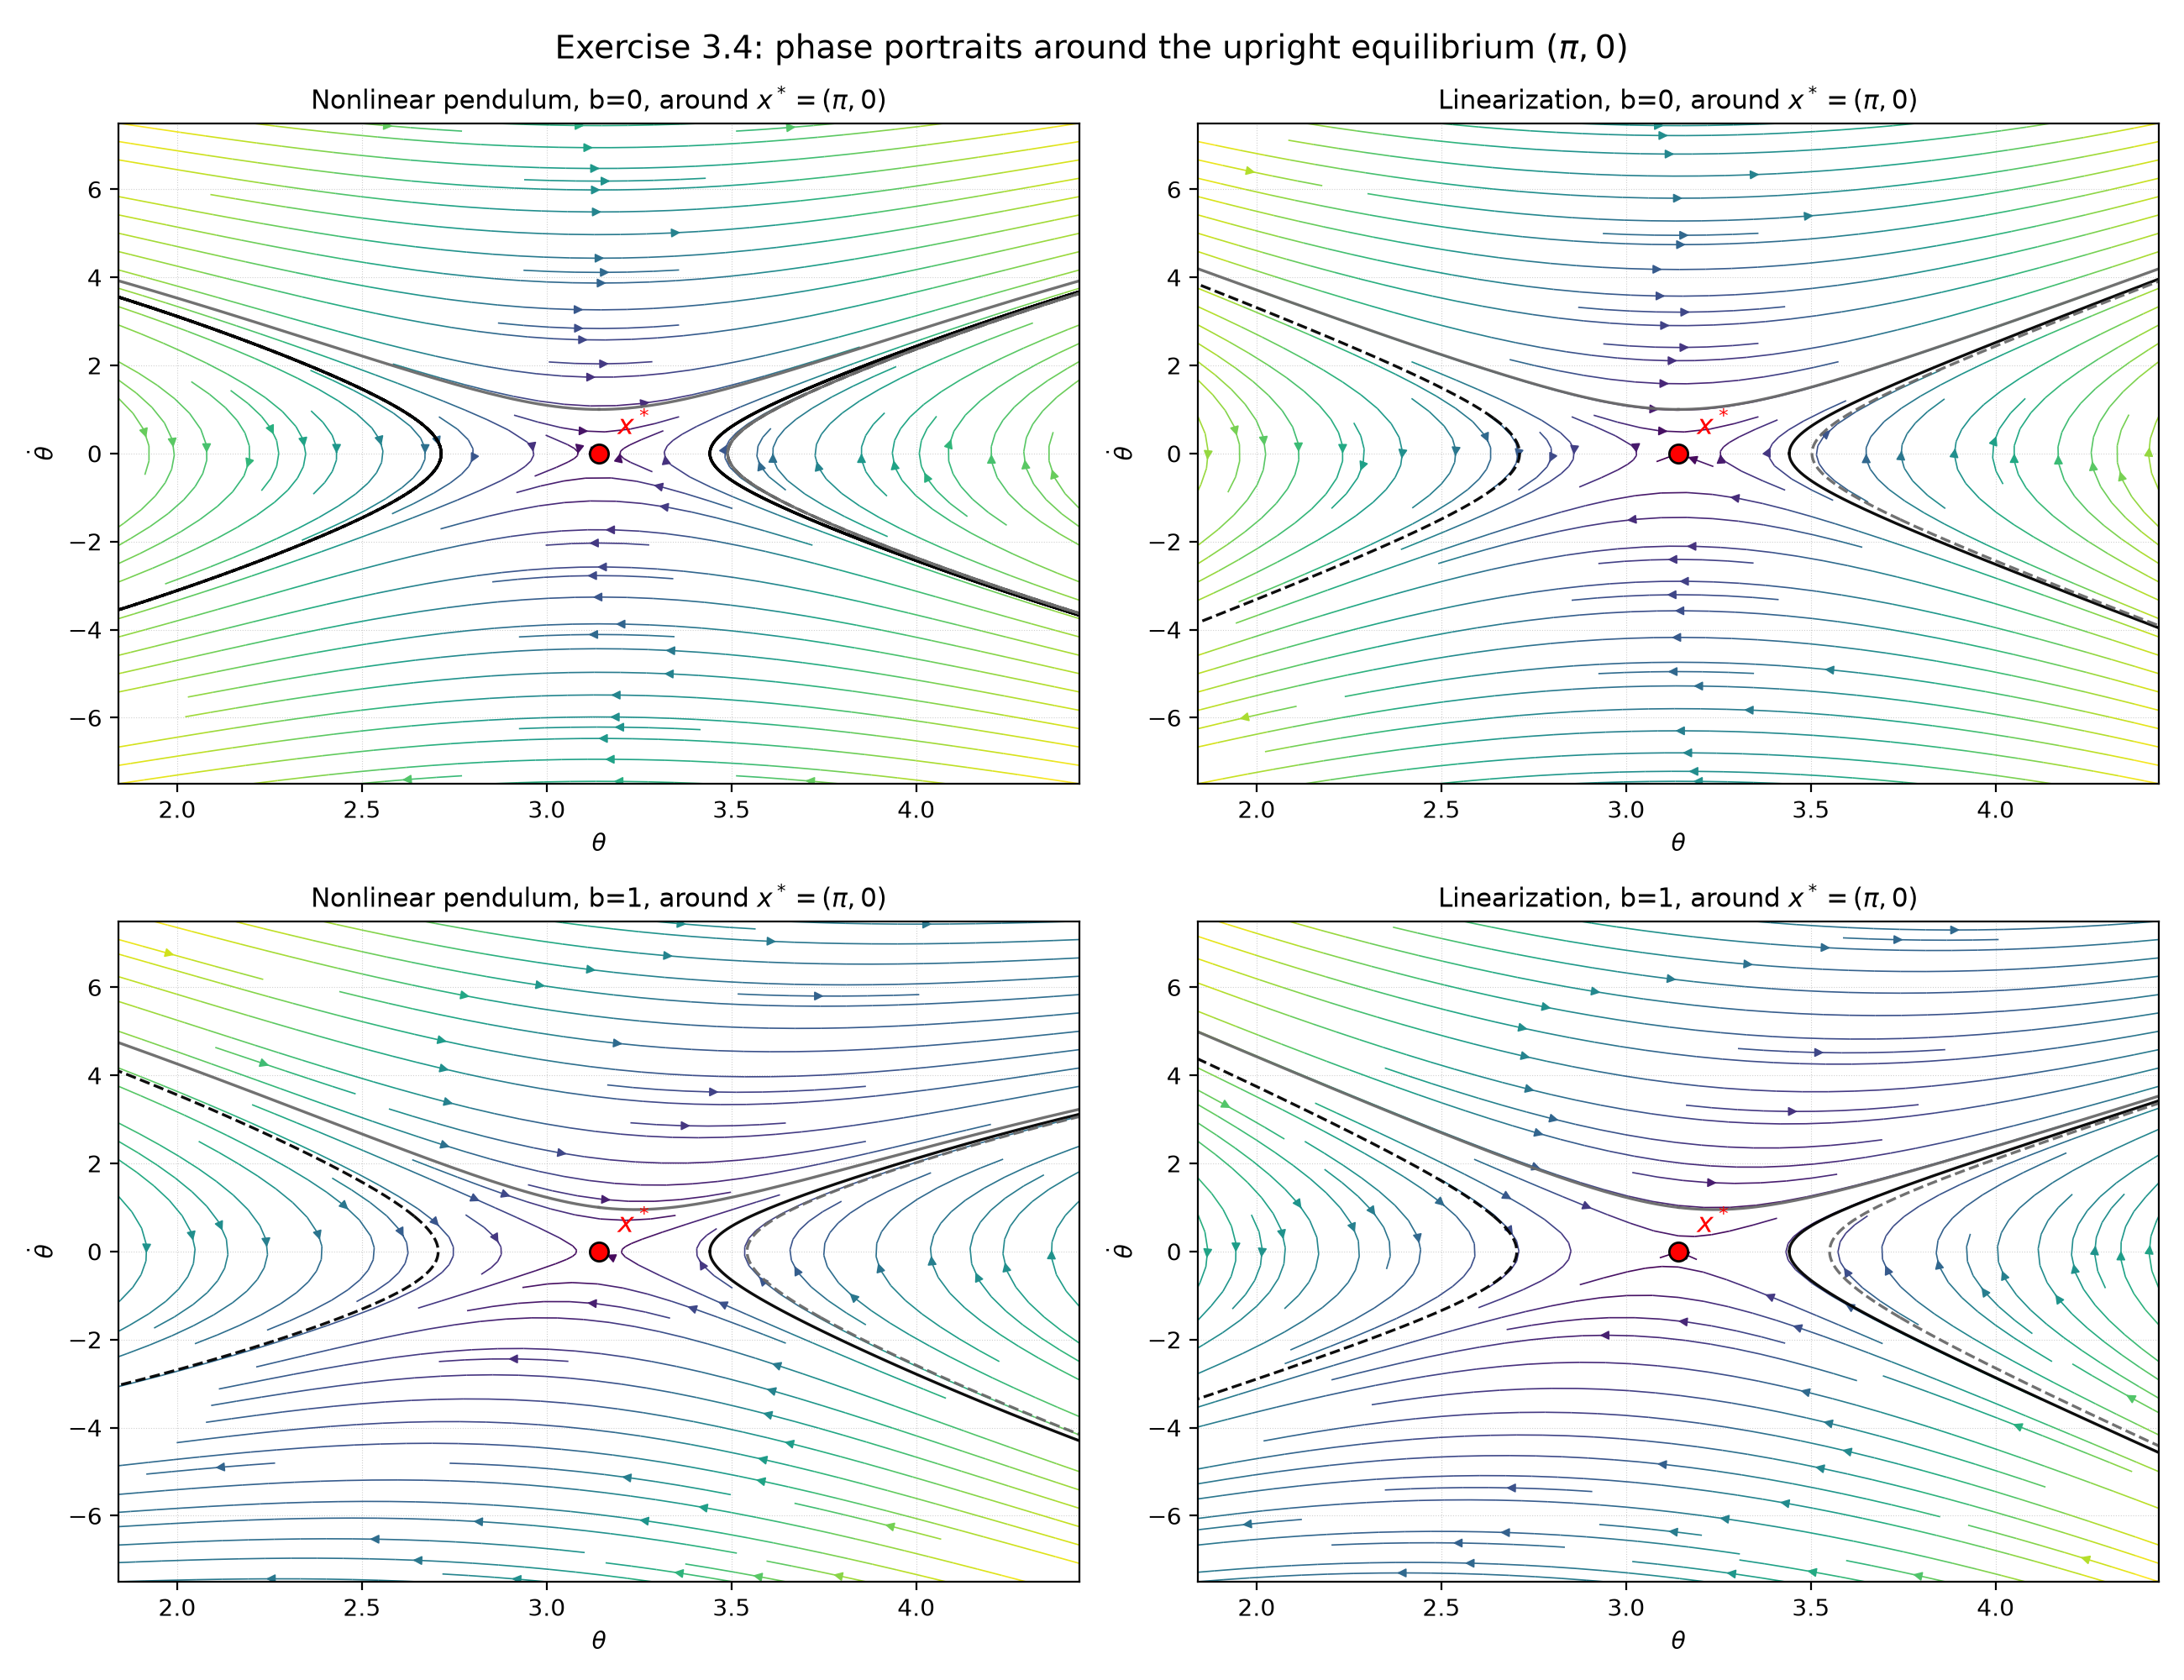
\includegraphics[width=0.9\textwidth]{ch3_phase_up.png}
\caption{Phase portraits around the upright equilibrium for $b=0$ (top) and
$b=1$ (bottom).  The stable manifold separates initial conditions that fall
left from those that fall right; damping does not remove the saddle.}
\end{figure}

\section{Implementation notes}

I ran the three example notebooks and the two exercise notebooks in the
environment described in the introduction.  The Monte-Carlo studies use fixed
seeds and 100 trials; the force and torque limits are stated with each table.
The acrobot and cart-pole parameters are the defaults from Drake and the
\texttt{underactuated} package.  For the quadrotor, the planar notebook was run
headlessly and the 3D notebook uses the official stabilising controller; the
sensitivity numbers come from \texttt{quadrotor\_analysis.py}.  The supplied
controller equations were not changed; the additional code is logging and the
loop over random initial conditions.

\section{Discussion}

The three examples share a workflow, but they fail in different ways.  The
acrobot and cart-pole are limited by saturation and by the non-minimum-phase
undershoot; the quadrotor is limited by the absence of integral action under a
constant wind.  The Section~3.8 exercises show that the linear model is local:
at $\theta=\pi/2$ the linearisation error is already larger than the field
itself.  A natural next step would be a swing-up controller for the acrobot and
cart-pole and an integral or MPC layer for the cart and quadrotor.  These are
outside the scope of this assignment, but they explain why the local LQR
results should not be read as global controllers.

%=====================================================================
\chapter{Simple Models of Walking and Running}
%=====================================================================

\section{Example 4.3: The Rimless Wheel}

The rimless wheel has $n=8$ spokes, no rim, a point mass at the hip, radius
$l=1$ and slope $\gamma$ \cite{tedrake-simplelegs}.  During stance it behaves as a simple pendulum,
\[
\ddot\theta=\frac{g}{l}\sin\theta,
\]
with energy $E=\frac12ml^2\dot\theta^2+mgl\cos\theta$.  At each foot strike
the new spoke becomes the stance leg and the collision map is
\[
\dot\theta^+=\dot\theta^-\cos(2\alpha).
\]
For $\alpha=\pi/8$ the kinetic energy is multiplied by $1/2$ at every step.
The step-to-step return map is
\[
\omega_{n+1}=\cos(2\alpha)\sqrt{\omega_n^2+4\frac{g}{l}\sin\alpha\sin\gamma}.
\]
A step is possible only above
$\omega_1=\sqrt{2(g/l)[1-\cos(\gamma-\alpha)]}$.  The rolling fixed point is
\[
\omega^\star=\cot(2\alpha)\sqrt{4\frac{g}{l}\sin\alpha\sin\gamma},
\]
and its multiplier is $\cos^2(2\alpha)=1/2$.  The fixed point exists only if
it lies above the step threshold.

\begin{figure}[htbp]
\centering
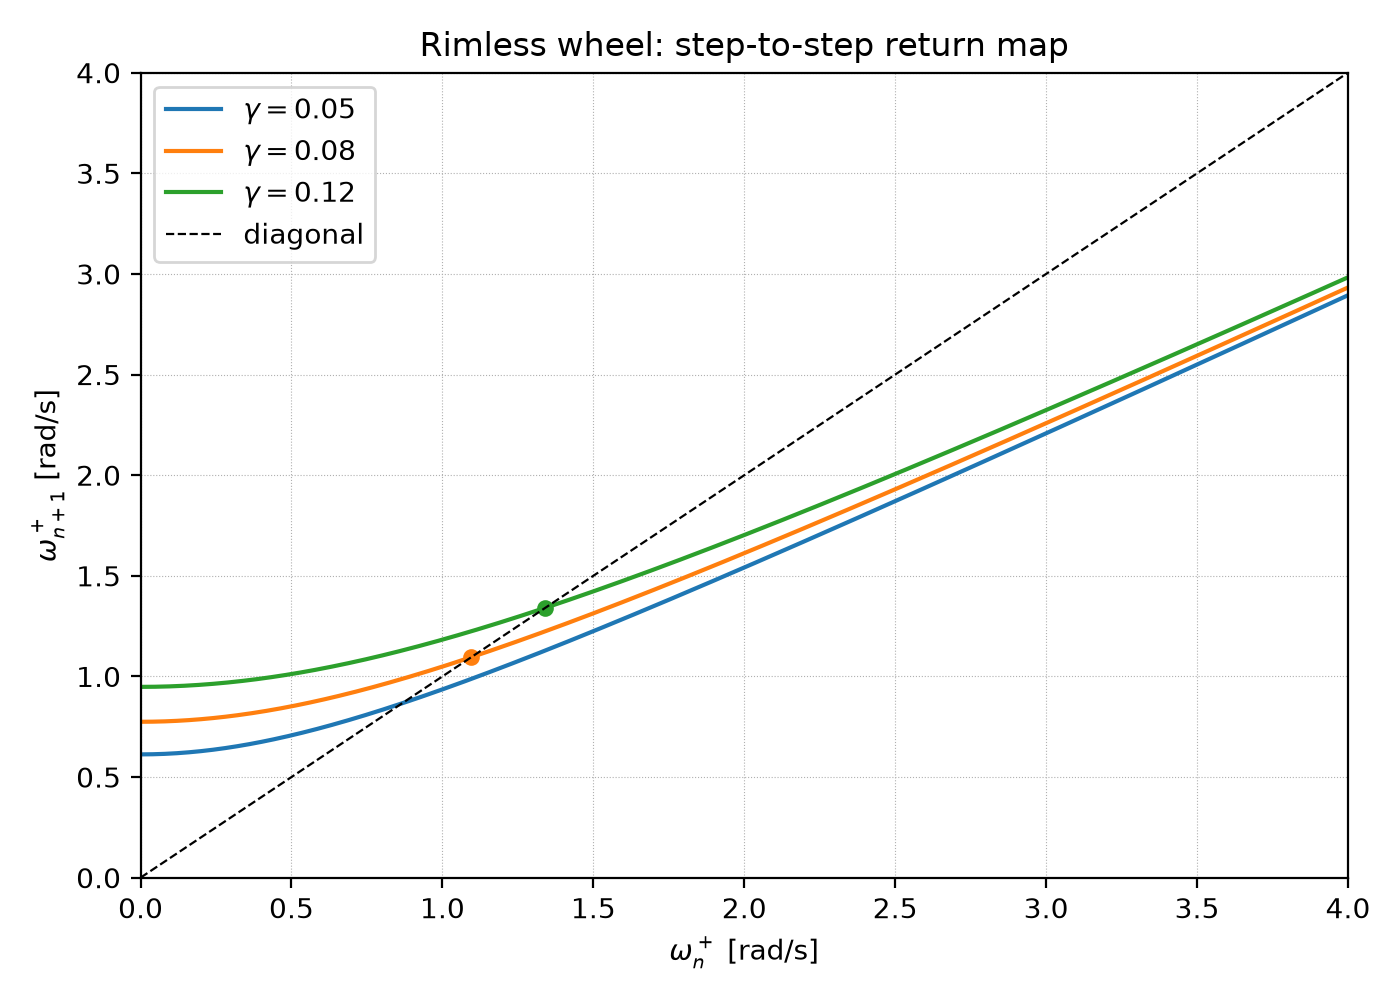
\includegraphics[width=0.72\textwidth]{ch4_rimless_return.png}
\caption{Rimless-wheel return map for three slopes.  Only slopes above about
0.067~rad have a fixed point above the step threshold; at 0.05~rad the wheel
cannot complete a step.}
\end{figure}

The slope study gives a clear threshold.  At $\gamma=0.02$ and $0.05$ the
fixed point is below $\omega_1$ and the wheel cannot sustain a rolling gait;
at $0.08$, $0.12$ and $0.20$ the fixed point is valid.  The multiplier is
$1/2$ in all cases, so the stability of the rolling gait is independent of the
slope once the fixed point exists.  The fixed point exists only where the gravity input per step can replace the
kinetic energy lost at impact; below that slope the map has no valid fixed
point.

\section{Example 4.4: The Compass Gait}

The compass gait has two point-mass legs of mass $m=5$~kg and length $l=1$~m
($a=b=0.5$~m), and a hip of mass $m_h=10$~kg.  The state is
$[\theta_{st},\theta_{sw},\dot\theta_{st},\dot\theta_{sw}]$.  The stance foot
is pinned, the swing leg moves freely, and at heel strike the roles of the two
legs are swapped.  The textbook initial condition is
$[0,0,0.4,-2.0]^\top$ with zero hip torque and slope $\gamma=0.0525$~rad.

The phase portrait approaches a closed orbit.  A step detector based on the
plant's ``left support'' state counts 14 steps in 10~s, with a mean period of
0.735~s.  The post-impact states converge quickly to a neighbourhood of the
limit cycle.  The basin is narrow: in a four-initial-condition test only the
nominal state stayed bounded, and in a $3\times3$ grid of initial states only
3 of 9 runs reached a sustained gait at the shallow slopes; at $\gamma=0.08$
and $0.12$ none of the nine runs did.  The passive gait is therefore a valid
demonstration, but not a robust walking controller.

\begin{figure}[htbp]
\centering
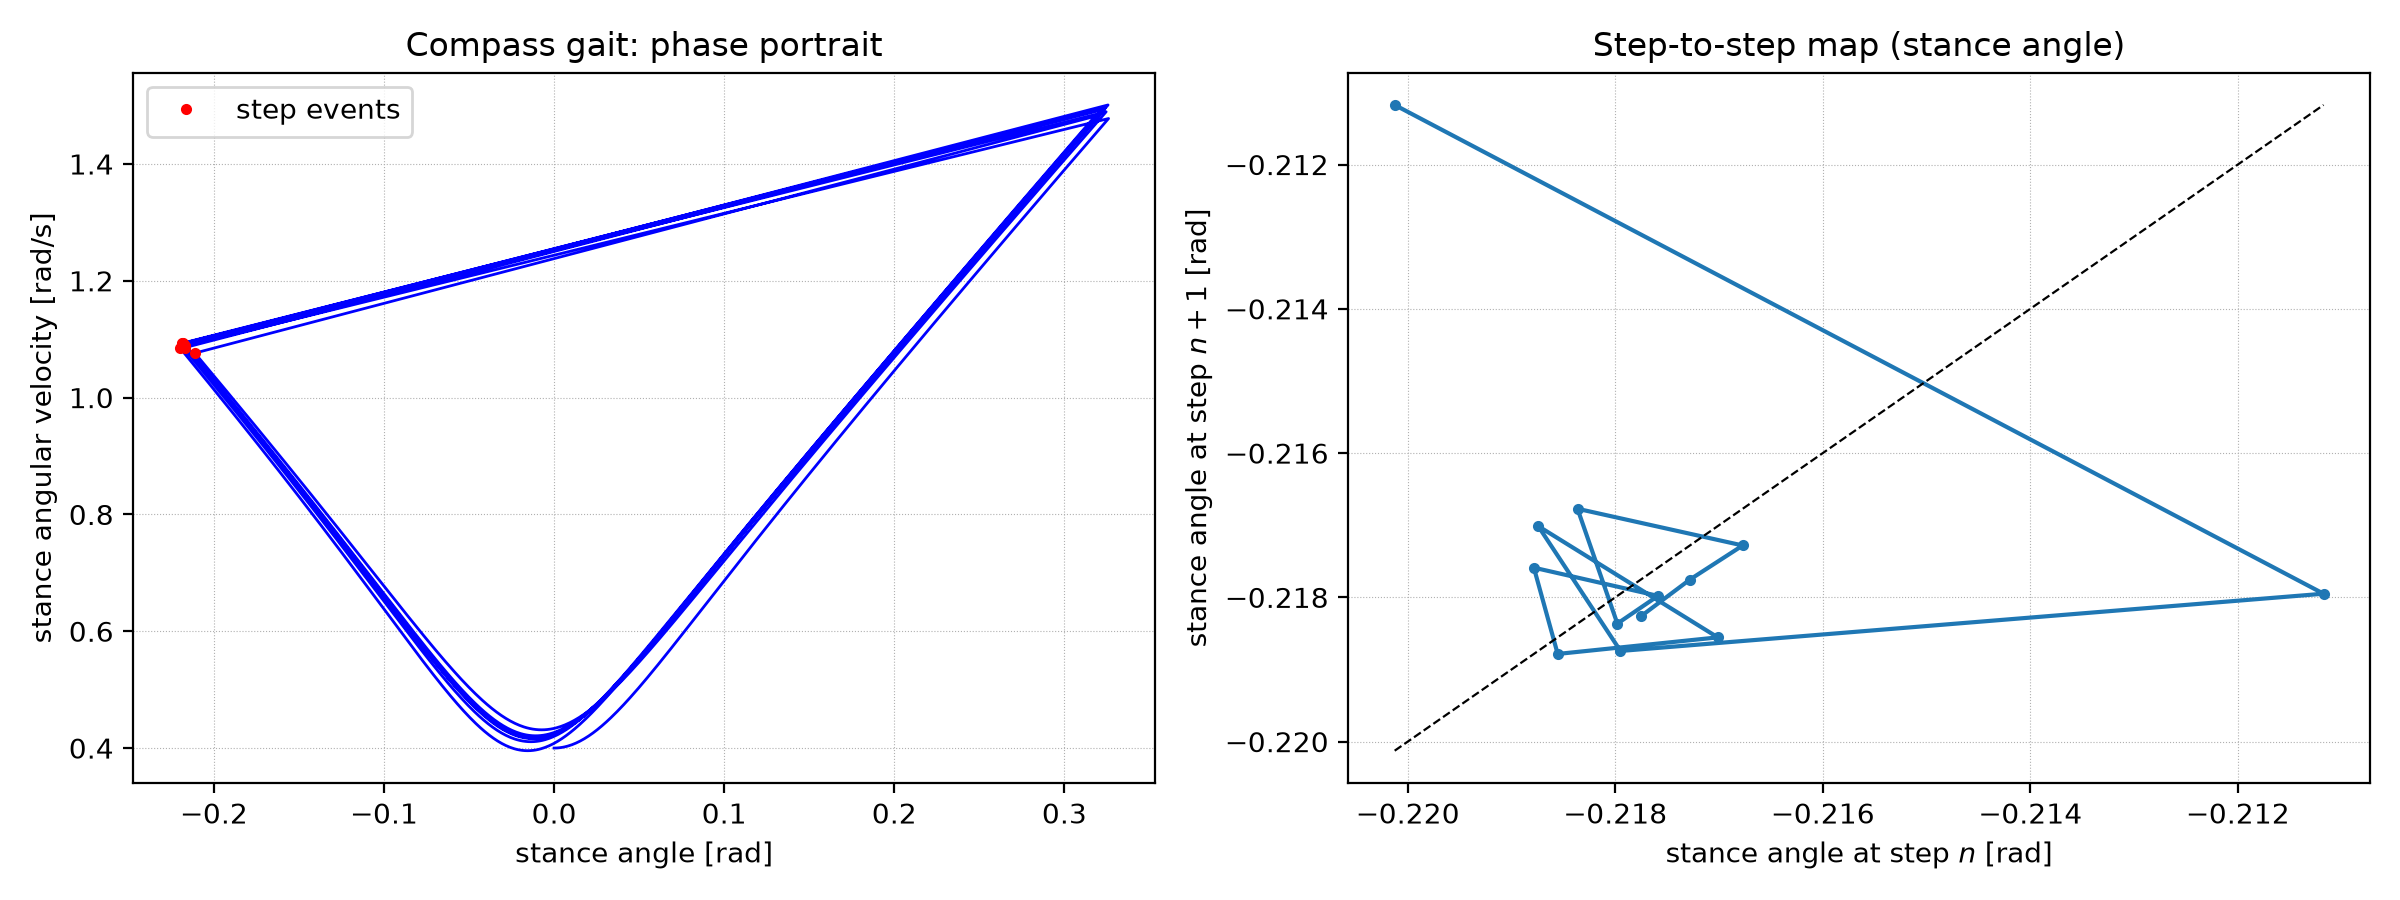
\includegraphics[width=0.85\textwidth]{ch4_compass_phase.png}
\caption{Compass gait: phase portrait and step-to-step map.  The step points
converge to the fixed point after the initial transient; perturbations outside
the narrow basin fall.}
\end{figure}

The contrast with the rimless wheel is instructive.  The wheel has many spokes
and a collision geometry that naturally returns the state to the rolling
solution.  The compass gait has only two legs, so the swing-leg landing must
match the previous step closely.  The energy balance can still produce a limit
cycle, but the basin is much smaller.

\section{Examples 4.5 and 4.6: SLIP and the Apex-to-Apex Map}

The spring-loaded inverted pendulum models running with a point mass, a
massless spring leg and a touchdown angle that is reset during flight.  In
flight the dynamics are ballistic; in stance,
\[
m\ddot r-mr\dot\theta^2+mg\cos\theta-k(r_0-r)=0,
\qquad
mr^2\ddot\theta+2mr\dot r\dot\theta-mgr\sin\theta=0.
\]
The mechanical energy
\[
E=\frac12m(\dot r^2+r^2\dot\theta^2)+mgr\cos\theta+\frac12k(r_0-r)^2
\]
is conserved because the leg and foot are massless.  Unlike the walking models, there is no impact loss; the spring stores and
returns the energy.

At the apex the vertical velocity is zero, and energy conservation makes the
horizontal velocity a function of the apex height.  The return map is
therefore one-dimensional, $z[n+1]=P(z[n])$.  For the nominal condition
$\theta_{td}=30^\circ$ and $\tilde E=1.61$ the stable fixed point is
$z^\star=0.8776$ with $P'=0.420$, and the unstable one is $z_u=0.9163$ with
$P'=1.288$.  The textbook values are $0.8768$ and $0.9168$, with derivatives
$0.488$ and $1.346$; the difference is due to the finite grid and linear
interpolation.

\begin{figure}[htbp]
\centering
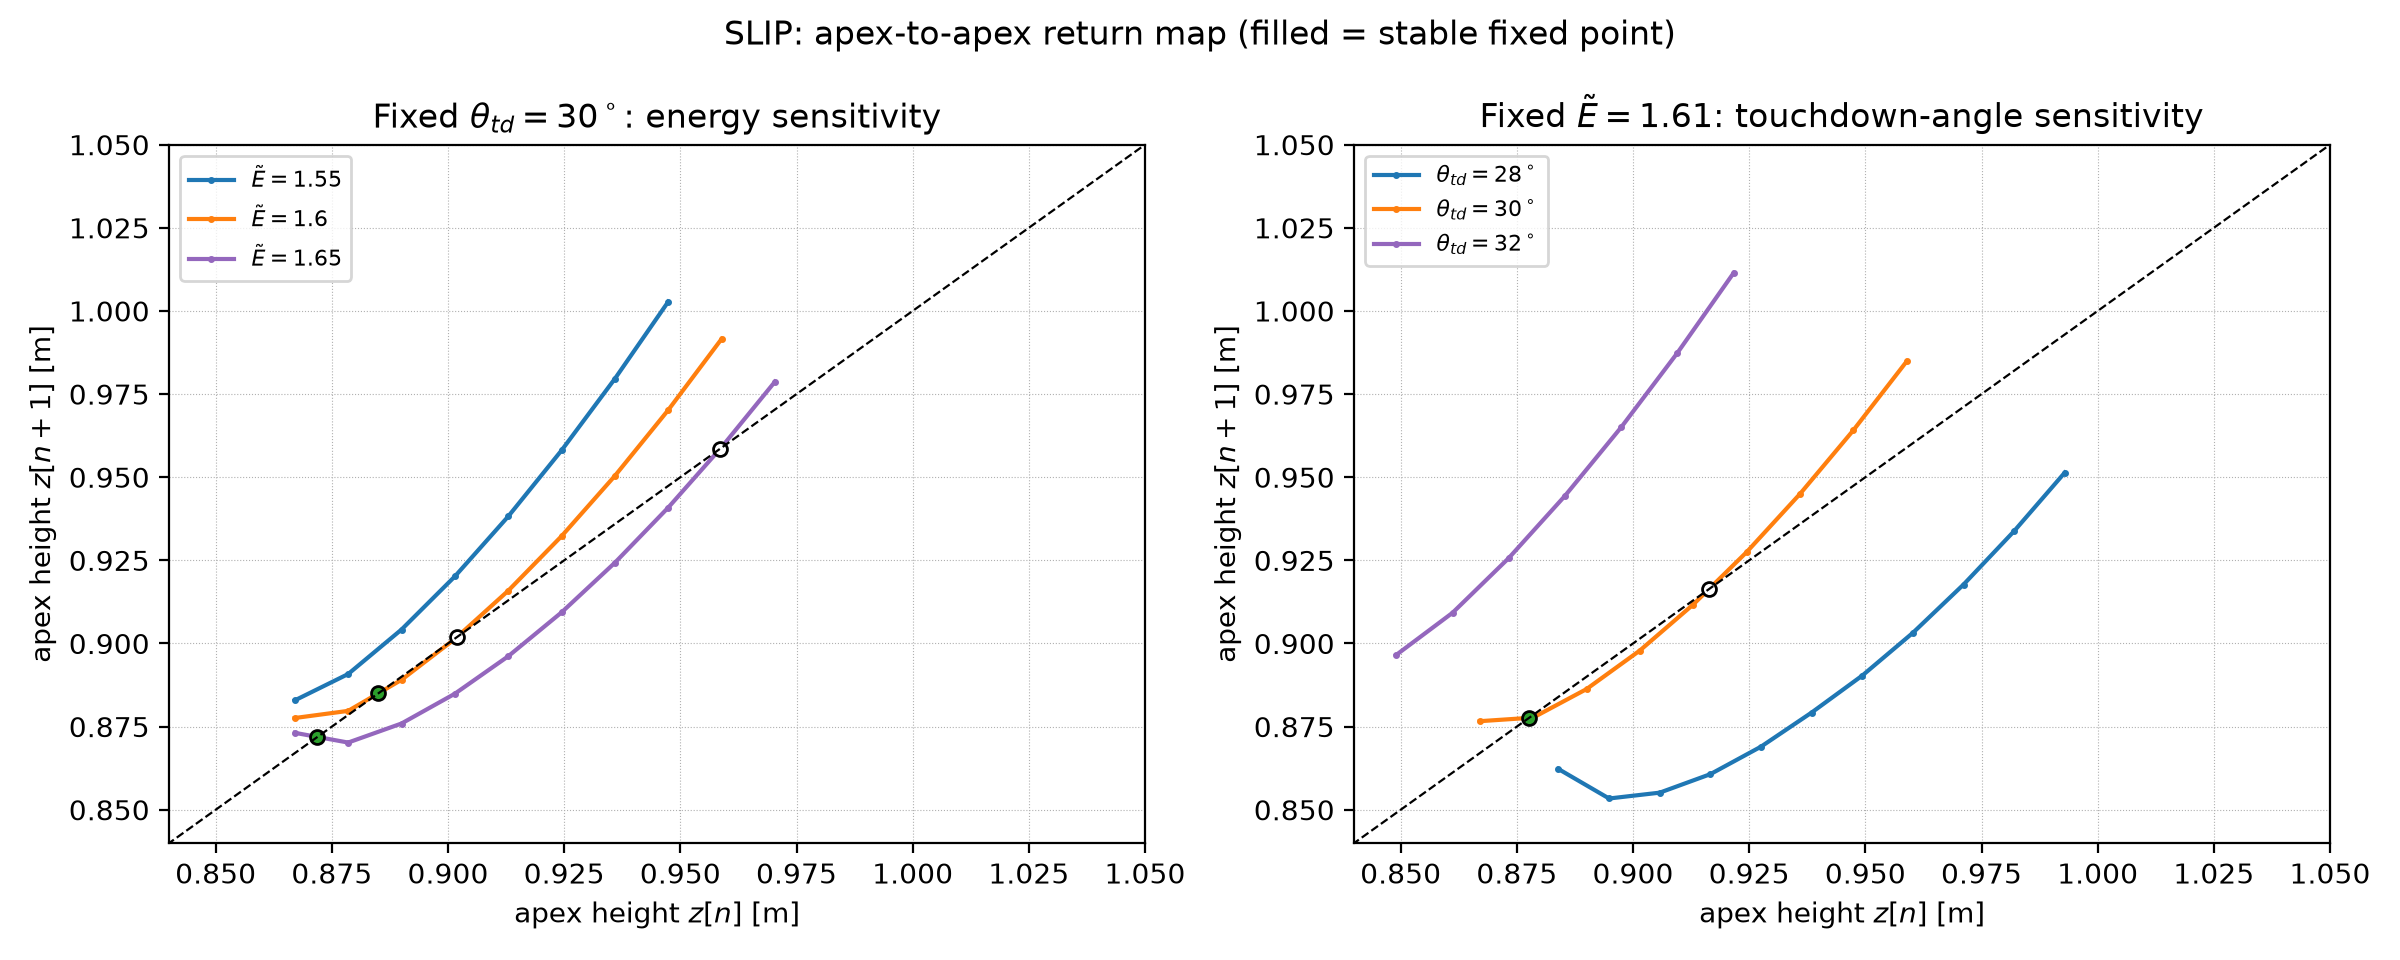
\includegraphics[width=0.9\textwidth]{ch4_slip_map.png}
\caption{SLIP apex-to-apex map.  The stable fixed point is at 0.8776~m with
$P'=0.42$; the unstable one is at 0.9163~m with $P'=1.29$.  Filled points are
stable fixed points.}
\end{figure}

The sensitivity study shows a narrow operating window.  At $30^\circ$ a stable
fixed point exists for $\tilde E=1.60,1.61,1.65$; changing the touchdown angle
to $28^\circ$ or $32^\circ$ removes the fixed point in the scanned range.  The
one-dimensional map is obtained on a constant-energy slice, so $|P'|<1$ proves
stability only for perturbations that preserve the energy.  Terrain changes
and pushes change the energy and are outside the map; this is the partial
stability discussed in the notes.  The apex map is useful for one-step
controllers, but a real robot still needs energy regulation.

\section{Section 4.6: The One-Dimensional Hopper}

The hopper has a body $m_b$, a leg $m_l$, a spring $k$ and a preload
$\delta\ge0$.  The state is $[z_b,l,\dot z_b,\dot l]$.  The controller changes
the preload twice per cycle: at the bottom it applies $\bar\delta$, and at the
apex it resets the preload to zero.  The mechanical energy is
\[
E=\frac12m_b\dot z_b^2+\frac12m_l(\dot z_b+\dot l)^2
+m_bgz_b+m_lg(z_b+l)+\frac12k(l+\delta)^2.
\]
Equating the energy at the bottom after the preload, at lift-off after the
inelastic impact, and at the apex gives
\[
\bar\delta=\frac12z_b+\frac{m_bg}{k}
-\frac{(m_b+m_l)^2}{k m_b z_b}gh.
\]
If this value is negative the system already has too much energy, and the
controller uses $\bar\delta=0$.

\begin{figure}[htbp]
\centering
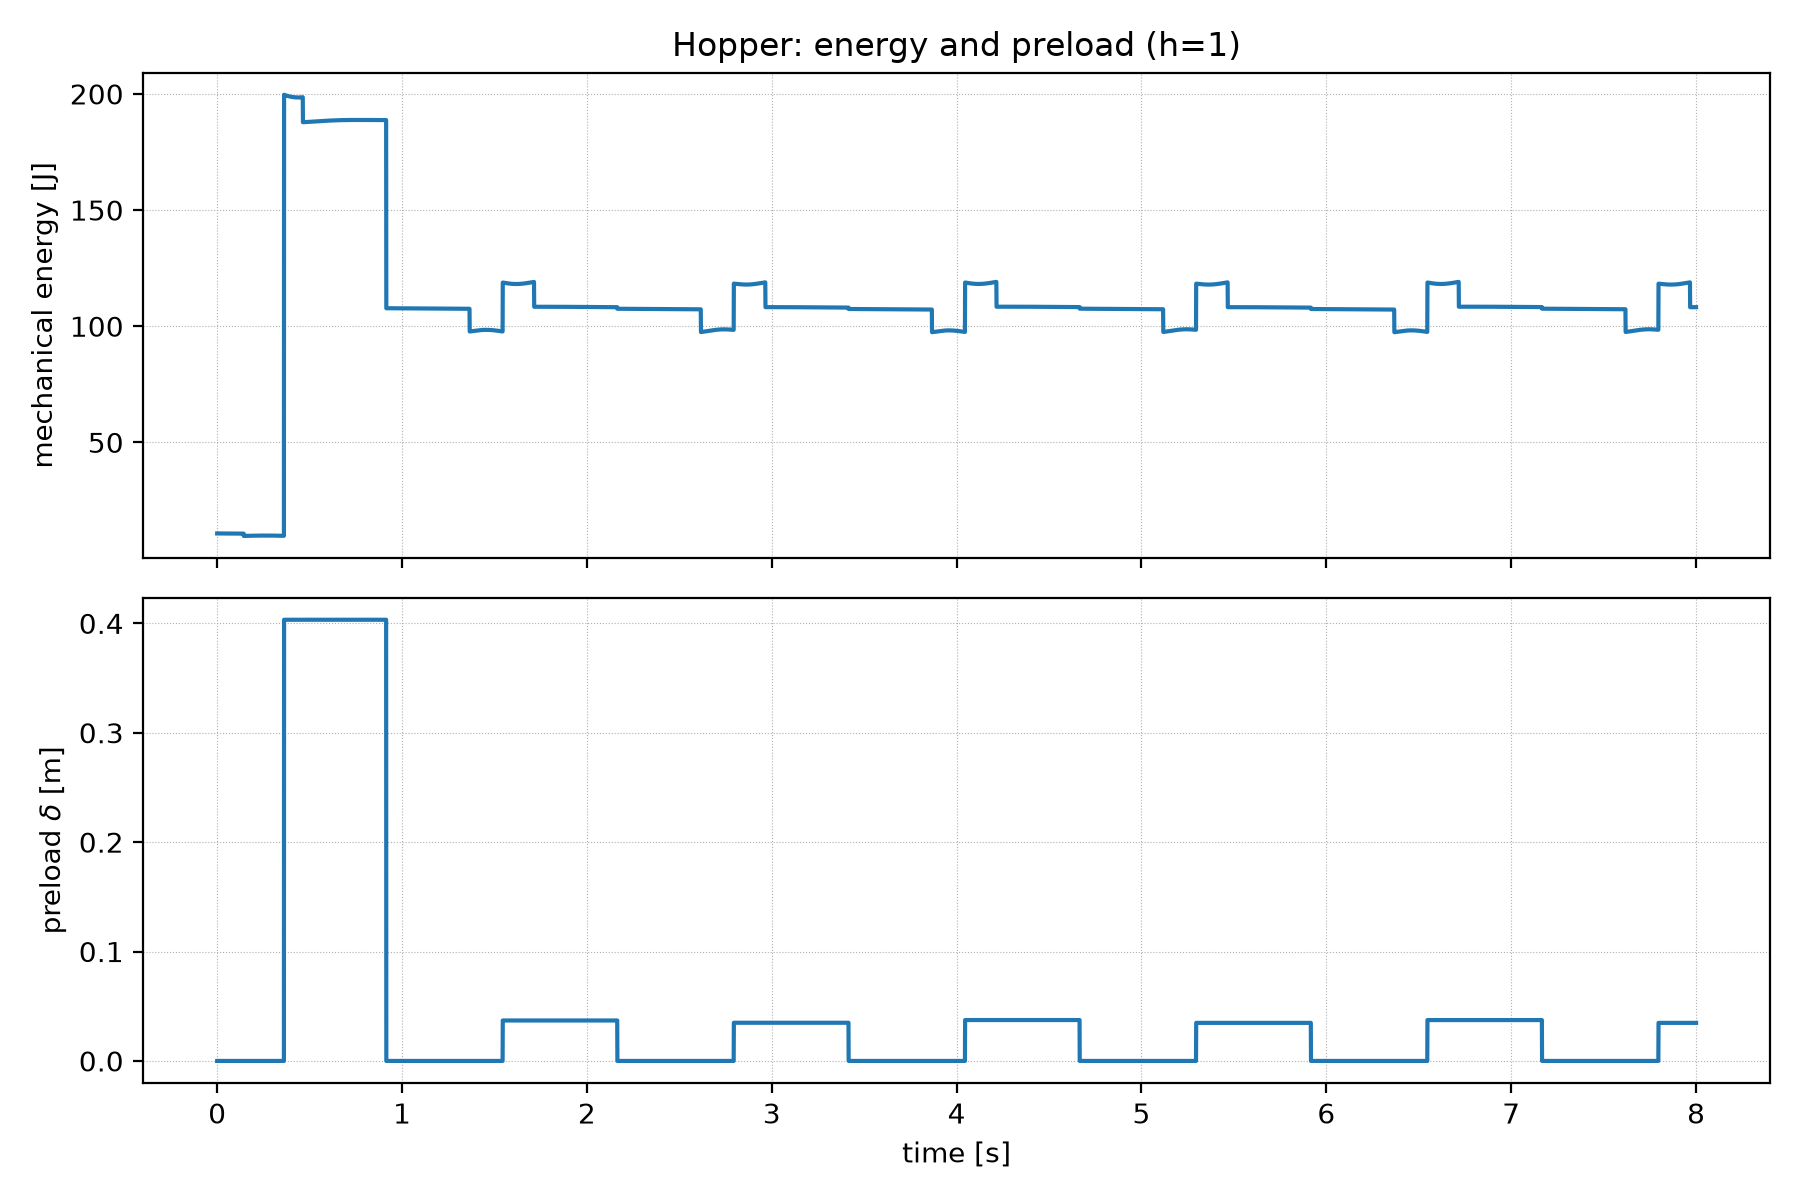
\includegraphics[width=0.9\textwidth]{ch4_hopper_energy.png}
\caption{Hopper energy and preload for $h=1$~m.  The two energy drops are the
touchdown and lift-off impacts; the preload pulses at the bottom restore the
energy.}
\end{figure}

The controller is implemented as a \texttt{LeafSystem} that detects the bottom
and apex by a sign change of $\dot z_b$ and sets the preload accordingly.  The
autograder gives 13/13.  In an 8~s simulation the final-two-second maximum
height is within 6~mm of the target for $h=0.5,0.75,1.0,1.25,1.5$~m.  The
maximum preload grows from about 0.024 to 0.302~m over this range, as expected
from the energy balance.  The controller is also insensitive to the initial
body height: starting from $z_b(0)=0.1$ to 1.0~m, the steady hopping height is
the same.

\section{Implementation notes}

I used the supplied rimless-wheel, compass-gait and SLIP notebooks and
implemented the hopper controller.  Steps in the compass gait are detected from
the plant's ``left support'' state; the rimless return map is computed from the
formula in the notebook; the SLIP map uses the notebook's
\texttt{SpringLoadedInvertedPendulum}.  The hopper controller computes the
preload at the bottom and resets it at the apex; the autograder gives 13/13.
For the hopper sensitivity, each run is 8~s and the last 2~s are used for the
height statistics.

\section{Discussion}

The passive walkers and SLIP illustrate two different stability mechanisms.
The rimless wheel and the compass gait rely on impact dissipation, and their
basins are set by the collision geometry; the compass gait's basin is much
narrower because it has only two legs.  SLIP has no impact loss, so the apex
map is conservative and the stability is only partial.  The hopper adds a
controller that restores the lost energy.  A limitation of these models
is the idealisation: point masses, no foot slip, no ground compliance, and, for
the hopper, one-dimensional motion.  A real robot would need a more detailed
contact model and a controller that handles terrain variation.

%=====================================================================
\chapter{Highly-articulated Legged Robots}
%=====================================================================

\section{Example 5.1: The ZMP Planner}

The first example is the ZMP planner for a humanoid \cite{tedrake-humanoids}.  The model is the linear
inverted pendulum, with the centre of mass at height $z_c$ and the zero-moment
point (ZMP) as the control point.  In the notebook the ZMP is tracked by a
linear controller; the nominal plan is a sequence of foot placements and a
reference ZMP.  The CoP identity is checked numerically and holds to machine
precision.  With the default weights the ZMP tracking error is about 0.153~m;
after a velocity push, the feedback policy reduces the final error to
$1.5\times10^{-5}$~m.  The timing sensitivity study shows that the tracking
error grows when the step timing is shortened, because the LIPM has less time
to move the CoM between supports.

\begin{figure}[htbp]
\centering
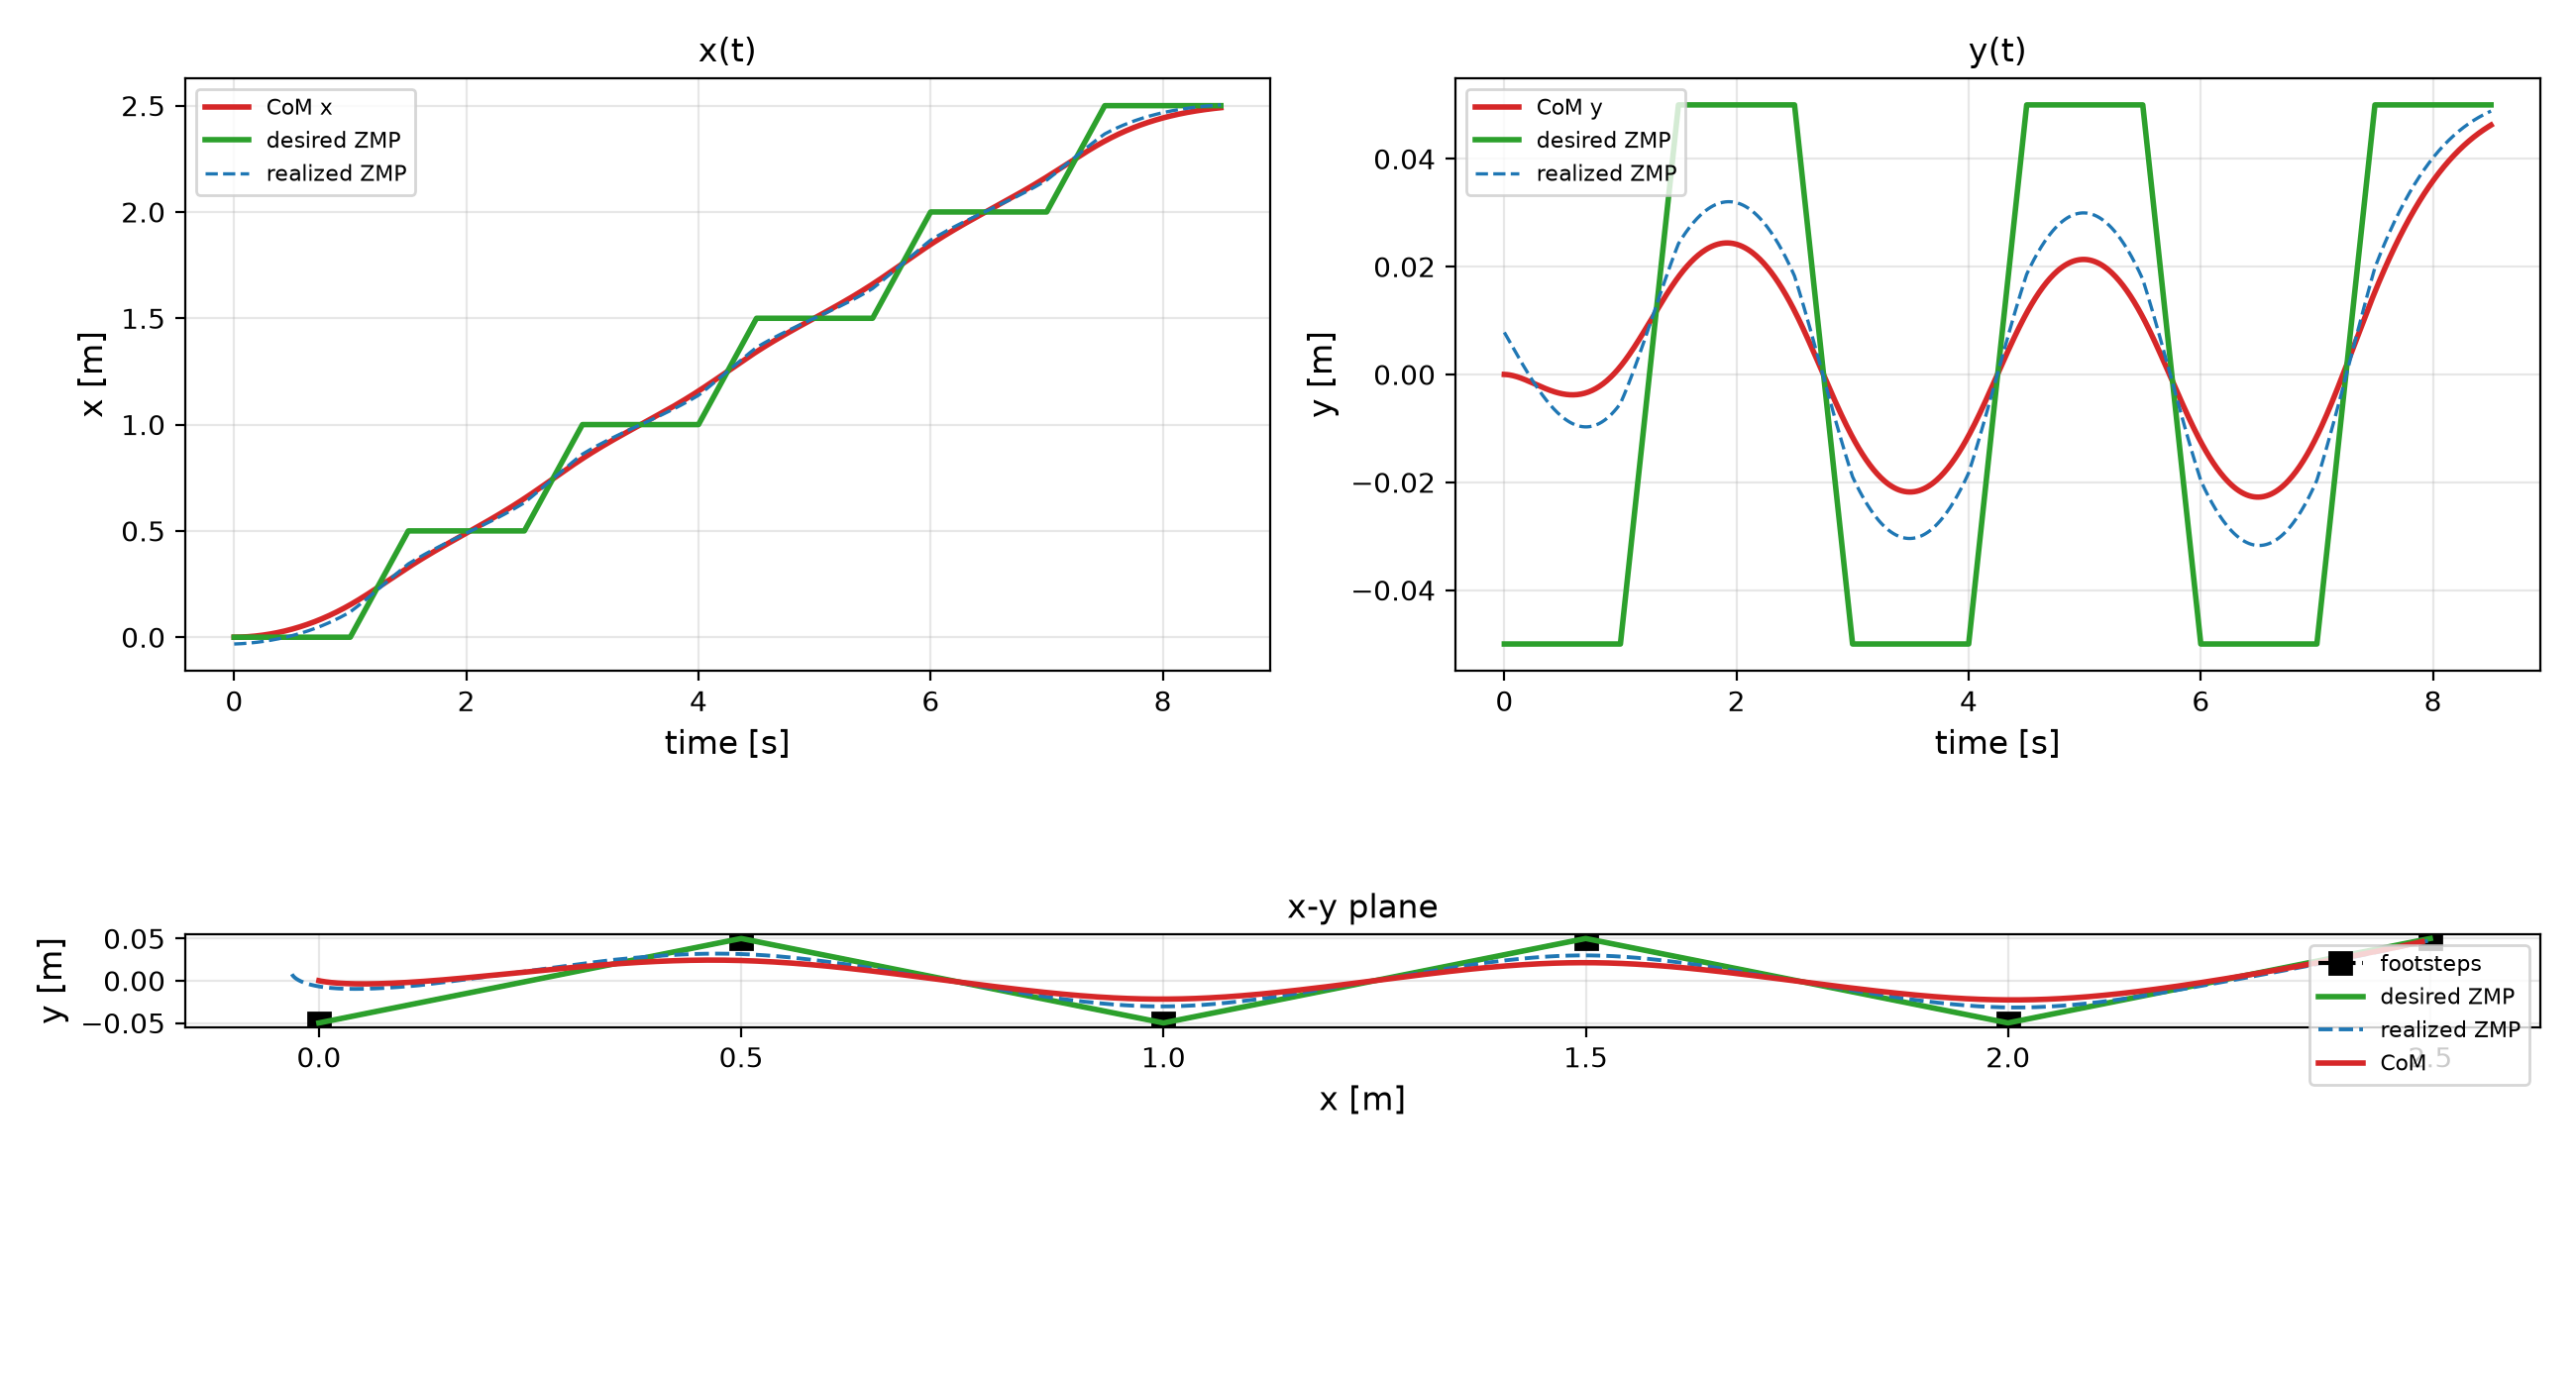
\includegraphics[width=0.85\textwidth]{ch5_zmp_plan.png}
\caption{ZMP planner: CoM and ZMP trajectories for the nominal footstep plan.
The default weights give a ZMP tracking error of 0.153~m; after a velocity push
the feedback run returns to \(1.5\times10^{-5}\)~m.}
\end{figure}

\section{Example 5.2: LittleDog Gait Optimization}

The second example optimises a walking gait for the LittleDog model.  The
decision variables are the gait timing and the contact schedule; the
constraints come from the centroidal dynamics and the foot geometry.  The
notebook uses SNOPT.  In the executed version the optimisation converges and
gives a stride period of about 0.6875~s and a CoM height between 0.131 and
0.148~m.  The result is a periodic gait with alternating support phases.  The gait is therefore an optimisation problem over contacts; the feedback
controller only tracks the resulting trajectory.

\begin{figure}[htbp]
\centering
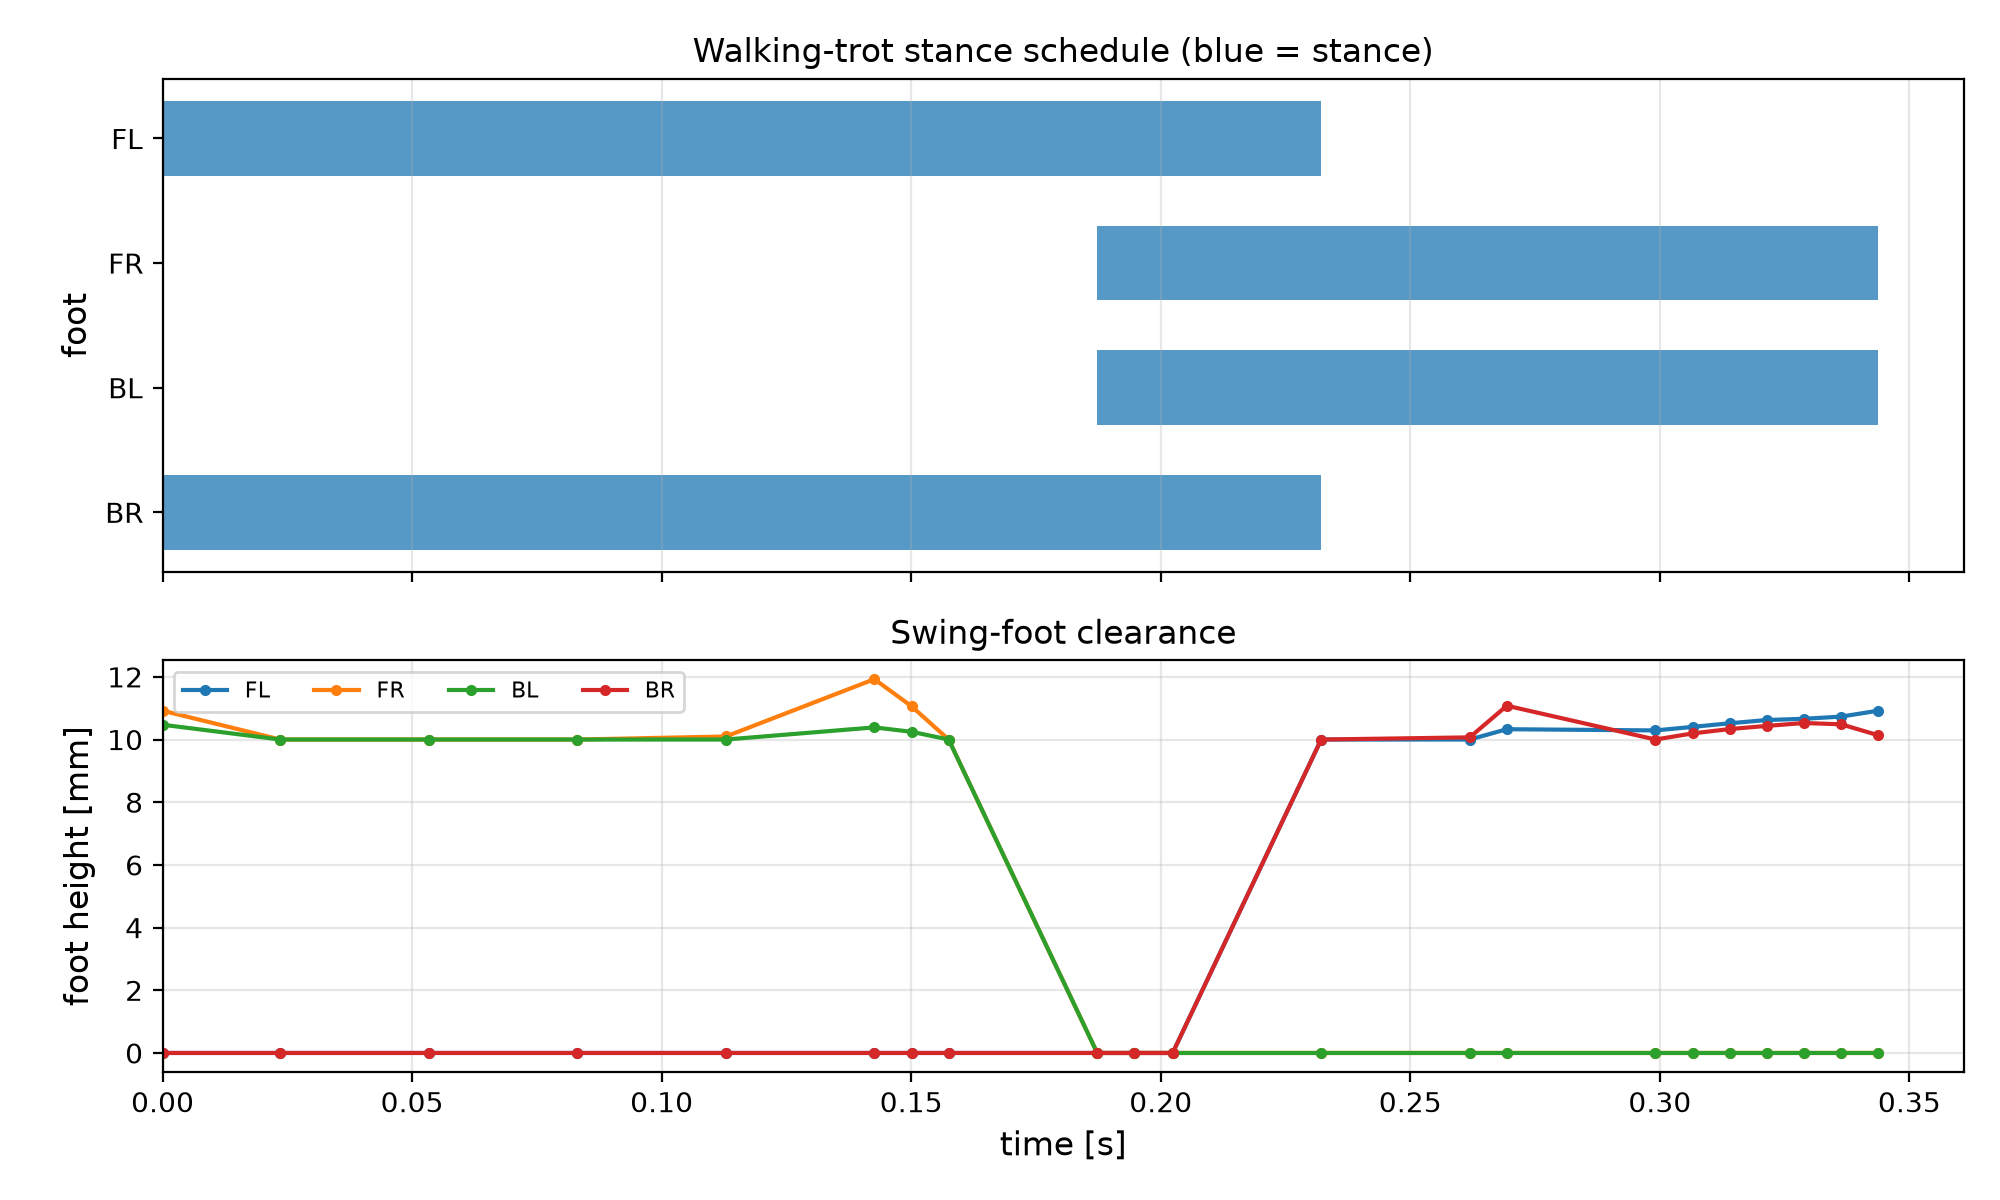
\includegraphics[width=0.9\textwidth]{ch5_littledog.png}
\caption{LittleDog gait: optimized contact schedule and body trajectory.  The
stride is 0.6875~s and the CoM height varies between 0.131 and 0.148~m.}
\end{figure}

\section{Section 5.8: Exercises 5.1--5.3}

The section contains three exercises.

\subsection{Exercise 5.1: Footstep Planning via MIQP}
The terrain and the footstep sequence are encoded with binary variables.  The
constraints enforce that each foot is assigned to one stepping stone, that the
relative foot positions are feasible, and that the chosen footholds are inside
the terrain.  The objective is the sum of the step lengths.  On the two
benchmark terrains the MIQP finds costs 4.1593 and 5.6721 and passes the
autograder 16/16.

\subsection{Exercise 5.2: Understanding the Zero-Moment Point}
This is an analytic exercise.  It derives the ZMP for a free-body diagram,
first without an ankle actuator and then with an ideal ankle actuator, and uses
the result to discuss foot design.  The ZMP is determined by the contact wrench and the CoM acceleration, not
simply by the centre of pressure; the ankle torque shifts it inside the support
polygon.  The exercise
also shows the range of motion of the actuated ankle for a given CoM
trajectory (about $76^\circ$ to $99^\circ$ in the numerical example).

\subsection{Exercise 5.3: Footstep Planning via GCS}
The GCS formulation represents the terrain as a graph of convex sets.  The
shortest path in the graph is found with a mixed-integer or convex
optimisation, and the result is a sequence of convex regions.  The GCS
solution uses 10-edge paths and passes the autograder 16/16.  Compared with
the MIQP, the GCS formulation is more structured and scales better when the
terrain can be decomposed into convex pieces; the MIQP is more direct for
small problems.

\begin{figure}[htbp]
\centering
\begin{subfigure}{0.48\textwidth}
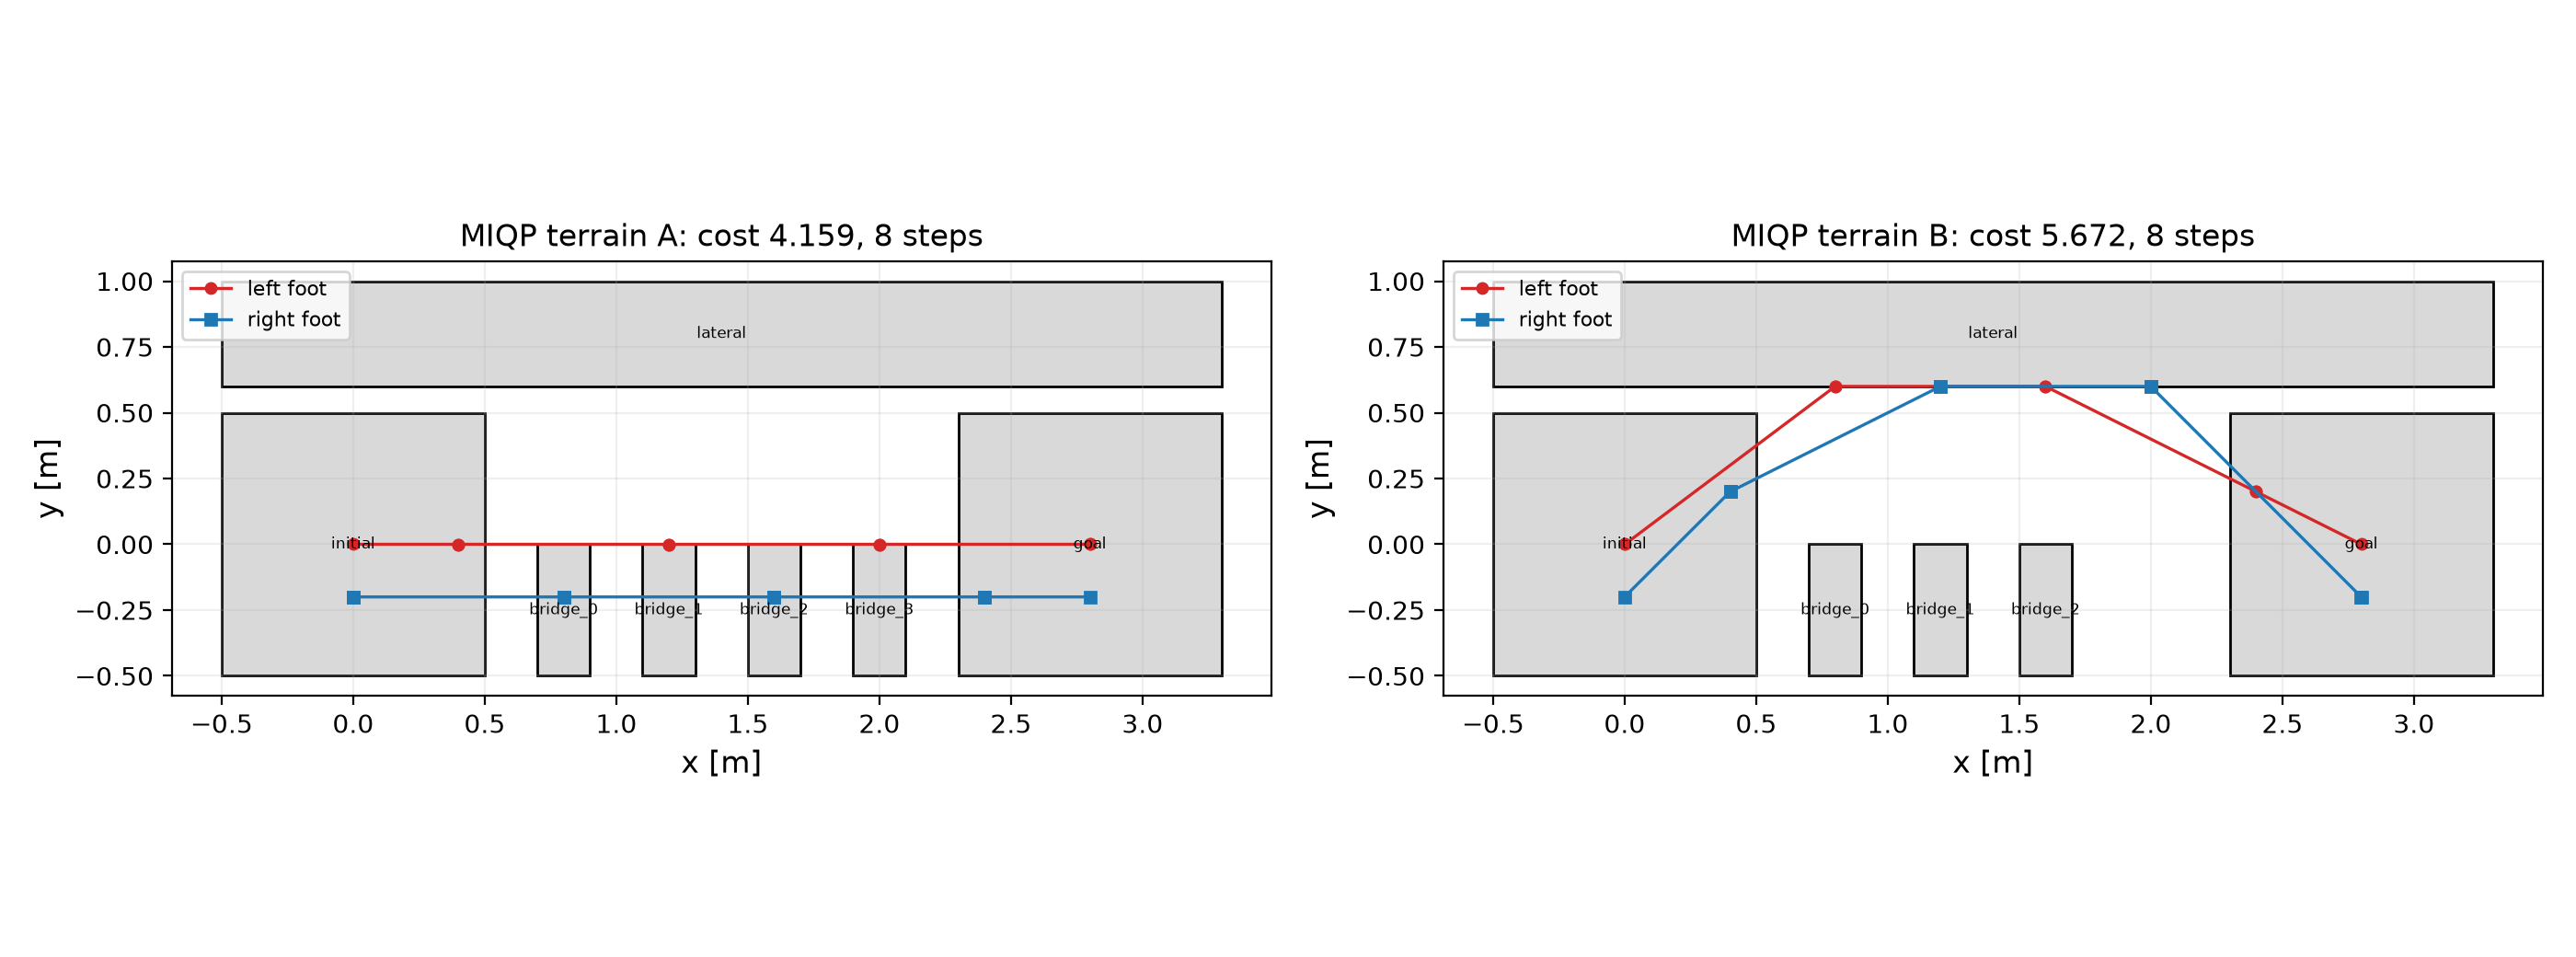
\includegraphics[width=\textwidth]{ch5_miqp.png}
\caption{MIQP footstep plan.}
\end{subfigure}\hfill
\begin{subfigure}{0.48\textwidth}
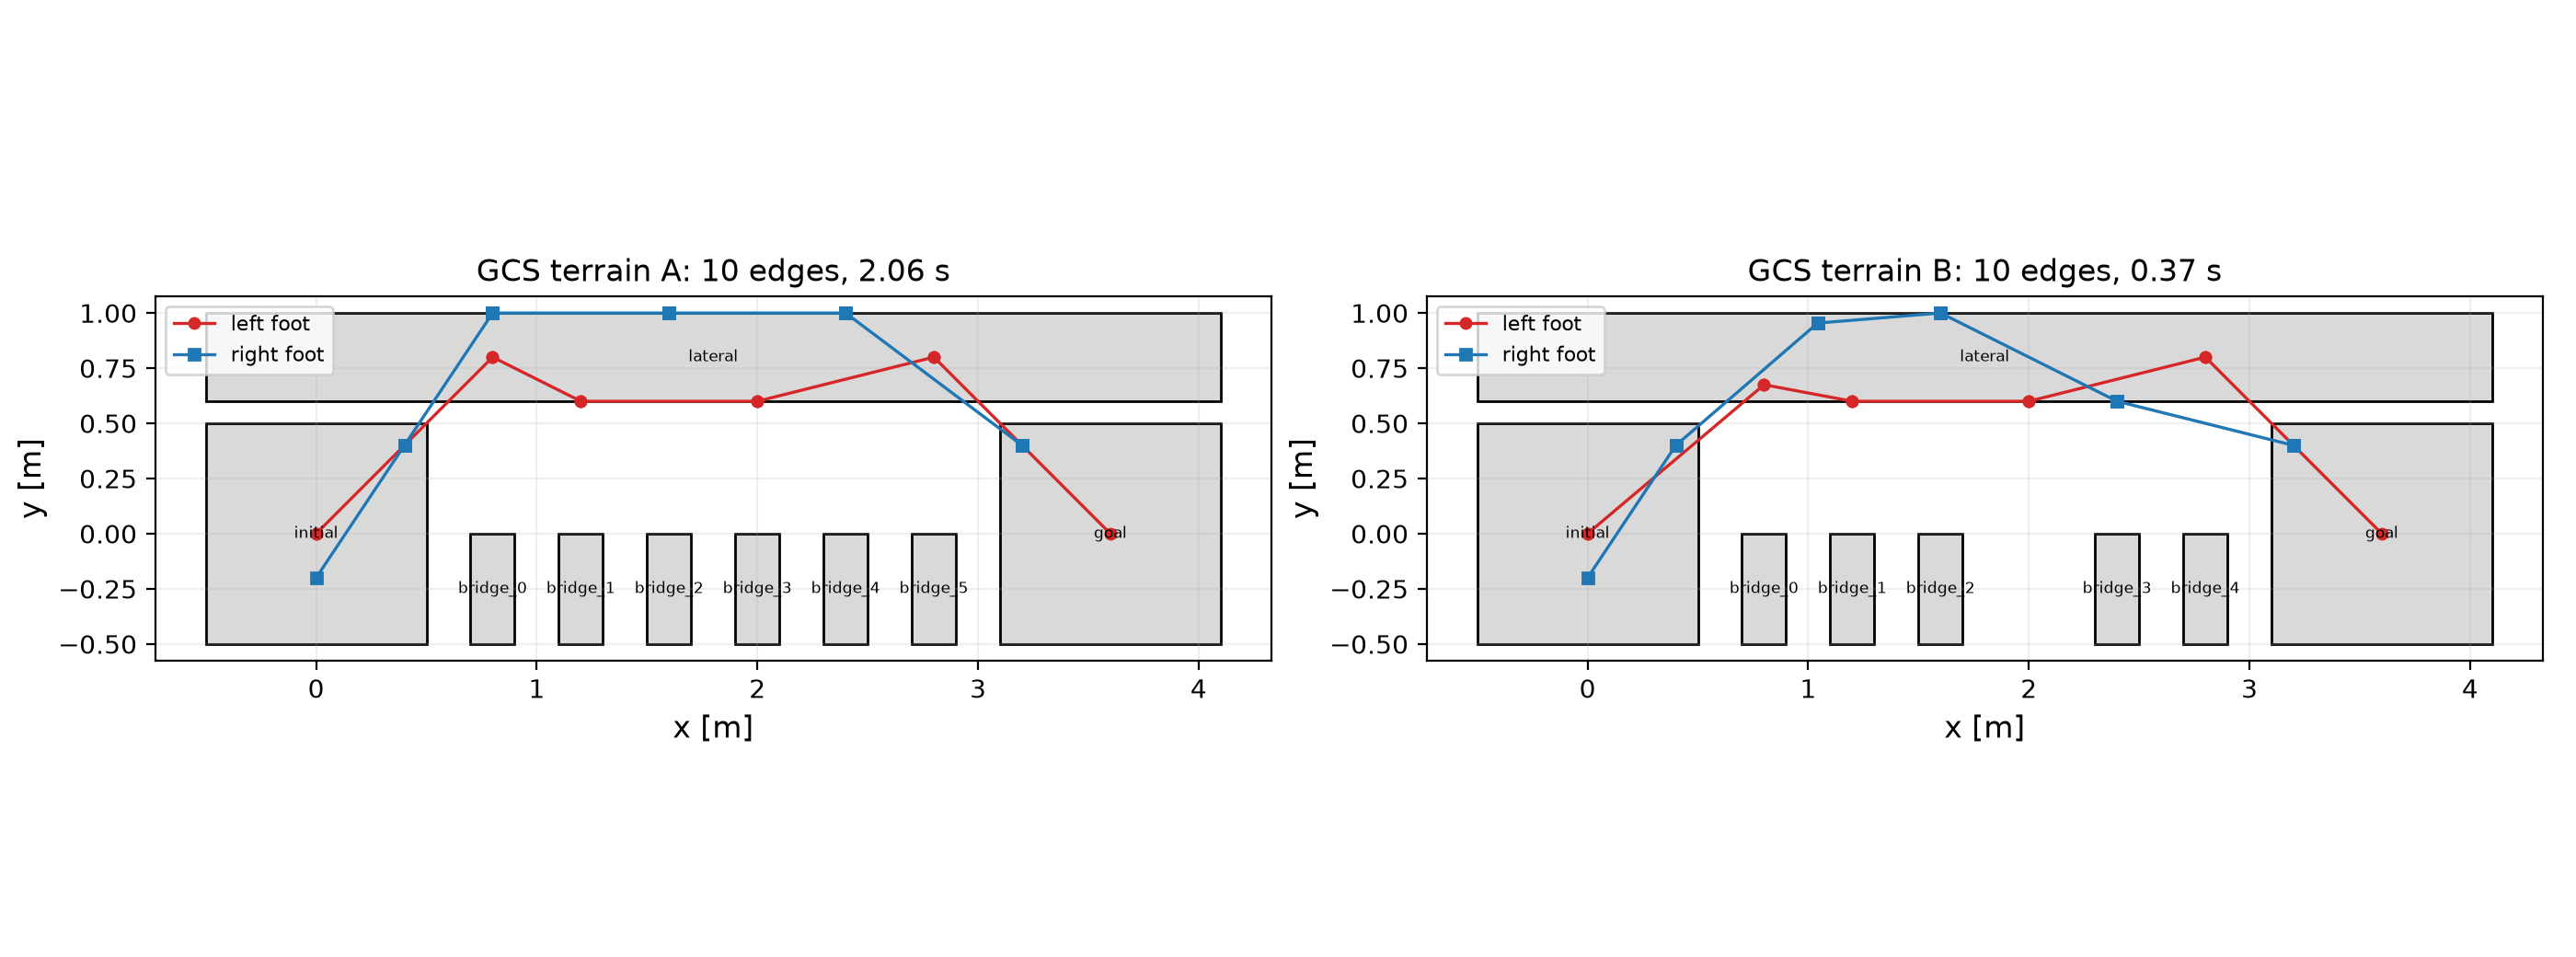
\includegraphics[width=\textwidth]{ch5_gcs.png}
\caption{GCS footstep plan.}
\end{subfigure}
\caption{Section 5.8 footstep plans on the benchmark terrains.  The MIQP costs
are 4.159 and 5.672 for terrains A and B; the GCS plans use 10 edges.}
\end{figure}

\section{Implementation notes}

I ran the ZMP and LittleDog notebooks and the two footstep-planning notebooks.
The LittleDog notebook's default SNOPT iteration limit was too small for the
gait to converge, so the major iteration limit was raised to 100; the reported
stride is 0.6875~s.  The MIQP and GCS exercises use the benchmark terrains in
the notebooks and pass 16/16 each.  The ZMP exercise is analytic; the numerical
values come from \texttt{zmp\_exercise\_analysis.py}.

\section{Discussion}

The ZMP planner, the LittleDog optimisation and the footstep planners address
different levels of the same problem.  The ZMP planner gives a CoM reference
but assumes a fixed contact sequence; the LittleDog optimisation chooses the
timing and contacts for a periodic gait; MIQP and GCS choose discrete
footholds.  The MIQP is direct but scales poorly with the number of steps; GCS
uses a convex decomposition and scales better, at the cost of a more structured
model.  The costs are sensitive to the solver settings and to the terrain
discretisation, so they should be read as benchmark values rather than
universal performance numbers.

%=====================================================================
\part{Manipulation}
%=====================================================================

%=====================================================================
\chapter{Introduction to Manipulation and Drake}
%=====================================================================

\section{Examples 1.1 and 1.2: Teleoperation in 2D and 3D}

The Manipulation introduction starts with teleoperation \cite{manipulation-intro}.  The notebook builds
a HardwareStation with an IIWA14 and a WSG gripper, adds a differential
inverse-kinematics block and connects a set of pose sliders.  The data flow is
simple: the sliders provide a desired end-effector pose, differential IK
converts it into joint positions, the station's position controller tracks
the joint command, and the measured pose is fed back to the sliders.

\begin{figure}[htbp]
\centering
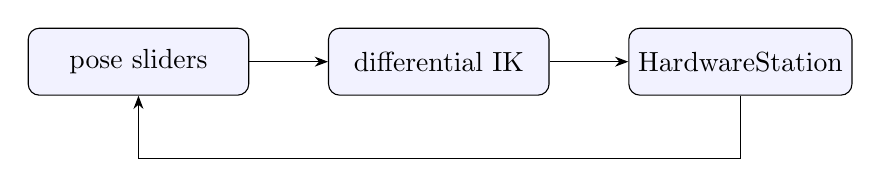
\begin{tikzpicture}[>=Stealth,node distance=1.0cm,
  box/.style={draw,rounded corners,align=center,fill=blue!5,
              minimum width=2.8cm,minimum height=0.85cm}]
  \node[box] (sliders) {pose sliders};
  \node[box,right=of sliders] (ik) {differential IK};
  \node[box,right=of ik] (station) {HardwareStation};
  \draw[->] (sliders)--(ik);
  \draw[->] (ik)--(station);
  \draw[->] (station.south) -- ++(0,-0.8) -| (sliders.south);
\end{tikzpicture}
\caption{Teleoperation data flow.  The sliders command a full pose, diff-IK
converts it to joint positions, and the measured pose is fed back.}
\end{figure}

\subsection{Background: Example 1.1 -- Teleoperation in 2D}

The 2D example restricts the visible task to roll, $x$ and $z$; the planar
IIWA14 has three actuated joints, so the task and the arm are matched in the
nominal configuration.

\subsection{Example 1.2: Teleoperation in 3D}

The 3D example uses the full 7-DoF IIWA14 and a 6-DoF pose slider.  The arm is now redundant: many joint configurations produce the
same end-effector pose, and differential IK chooses the one closest to the
current configuration.  In both cases the sliders and the gripper button are
the operator interface; the controller and the plant are hidden behind the
station ports.

The differential IK solves a local least-squares problem
\[
\min_{\dot q}\ \|J(q)\dot q-\dot X_d\|^2+\lambda\|\dot q\|^2
\]
subject to joint limits and integrates $\dot q$.  It is fast and degrades
gracefully: when a target is outside the workspace or near a singularity, the
solver reports \texttt{stuck} instead of producing a discontinuous jump.  The
3D demo also shows the limitation of purely kinematic teleoperation: the
clutter is not avoided, because obstacle avoidance is a separate layer.

\section{Example 1.3: System Diagrams}

The System Diagrams example makes the modelling paradigm explicit.  A
manipulation system is a \texttt{Diagram} of smaller systems, each with its own
state and ports.  The teleoperation demo is already such a diagram: a plant, a
controller, a visualizer, and a slider interface.  The interactive example
lets the reader expand the \texttt{iiwa\_controller} block and see the hidden
complexity inside a single box.

\begin{figure}[htbp]
\centering
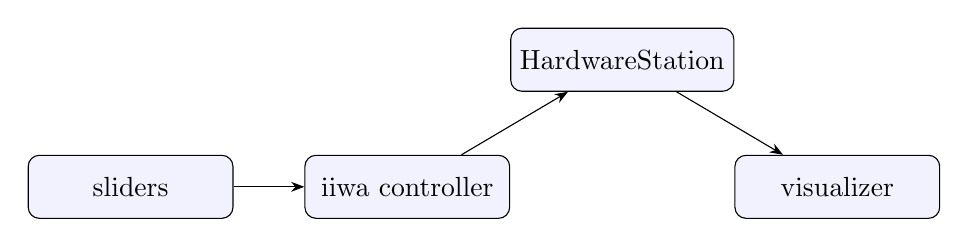
\begin{tikzpicture}[>=Stealth,node distance=0.8cm,
  box/.style={draw,rounded corners,align=center,fill=blue!5,
              minimum width=2.6cm,minimum height=0.8cm}]
  \node[box] (station) {HardwareStation};
  \node[box,below left=0.8cm and 0.0cm of station] (ctrl) {iiwa controller};
  \node[box,below right=0.8cm and 0.0cm of station] (vis) {visualizer};
  \node[box,left=0.9cm of ctrl] (sliders) {sliders};
  \draw[->] (sliders)--(ctrl);
  \draw[->] (ctrl)--(station);
  \draw[->] (station)--(vis);
\end{tikzpicture}
\caption{A system diagram in the spirit of Example~1.3.  The station is a nested
diagram; expanding the IIWA controller shows the position controller and model
driver inside.}
\end{figure}

The benefit of the block-diagram approach is composability: a controller,
filter or plant can be replaced without rewriting the rest of the system.  The
cost is that state and ports must be declared explicitly, which can feel like
overhead for a small script.  For a manipulation stack with perception,
planning, control and simulation, the structure is what keeps the parts
interchangeable.  The HardwareStation scenario used in Exercise~1.4 is a
declarative description of the same idea.

\section{Section 1.7: Exercises 1.1--1.4}

\paragraph{Exercise 1.1: Familiarize yourself with Drake.}
The three documentation questions have short answers:
\begin{enumerate}[leftmargin=1.4em,itemsep=2pt]
  \item In the \texttt{dynamical\_systems} tutorial \cite{drake-tutorials} the initial condition of
        \texttt{SimpleContinuousTimeSystem} is set to $x(0)=0.9$.
  \item In the C++ doxygen page on spatial vectors, angular acceleration is
        written \texttt{alpha}; angular velocity is \texttt{w}, torque is
        \texttt{t}, and the translational quantities are \texttt{v},
        \texttt{a} and \texttt{f}.
  \item The Python fitted-value-iteration unit test sets
        \texttt{options.convergence\_tol = 1.0}.  The default value of
        \texttt{DynamicProgrammingOptions} is \texttt{1e-4}, but the test
        deliberately uses the larger tolerance.
\end{enumerate}

\paragraph{Exercise 1.2: Drake Systems Fundamentals.}
The exercise implements an inverted pendulum as a \texttt{LeafSystem} with
state $[\theta,\dot\theta]$, a torque input and an angle output.  The dynamics
are $\ddot\theta=-g\sin\theta+\tau/(ml^2)$; for the default $m=l=1$ this is
$-9.81\sin\theta+\tau$.  The system is wired into a diagram with a constant
torque source and a logger, and simulated with Drake's \texttt{Simulator}.  The
two verification cases give $\theta(2.5)=0.0052$~rad and
$\theta(1.8)=-0.1074$~rad.  The autograder gives 70/70.

\begin{figure}[htbp]
\centering
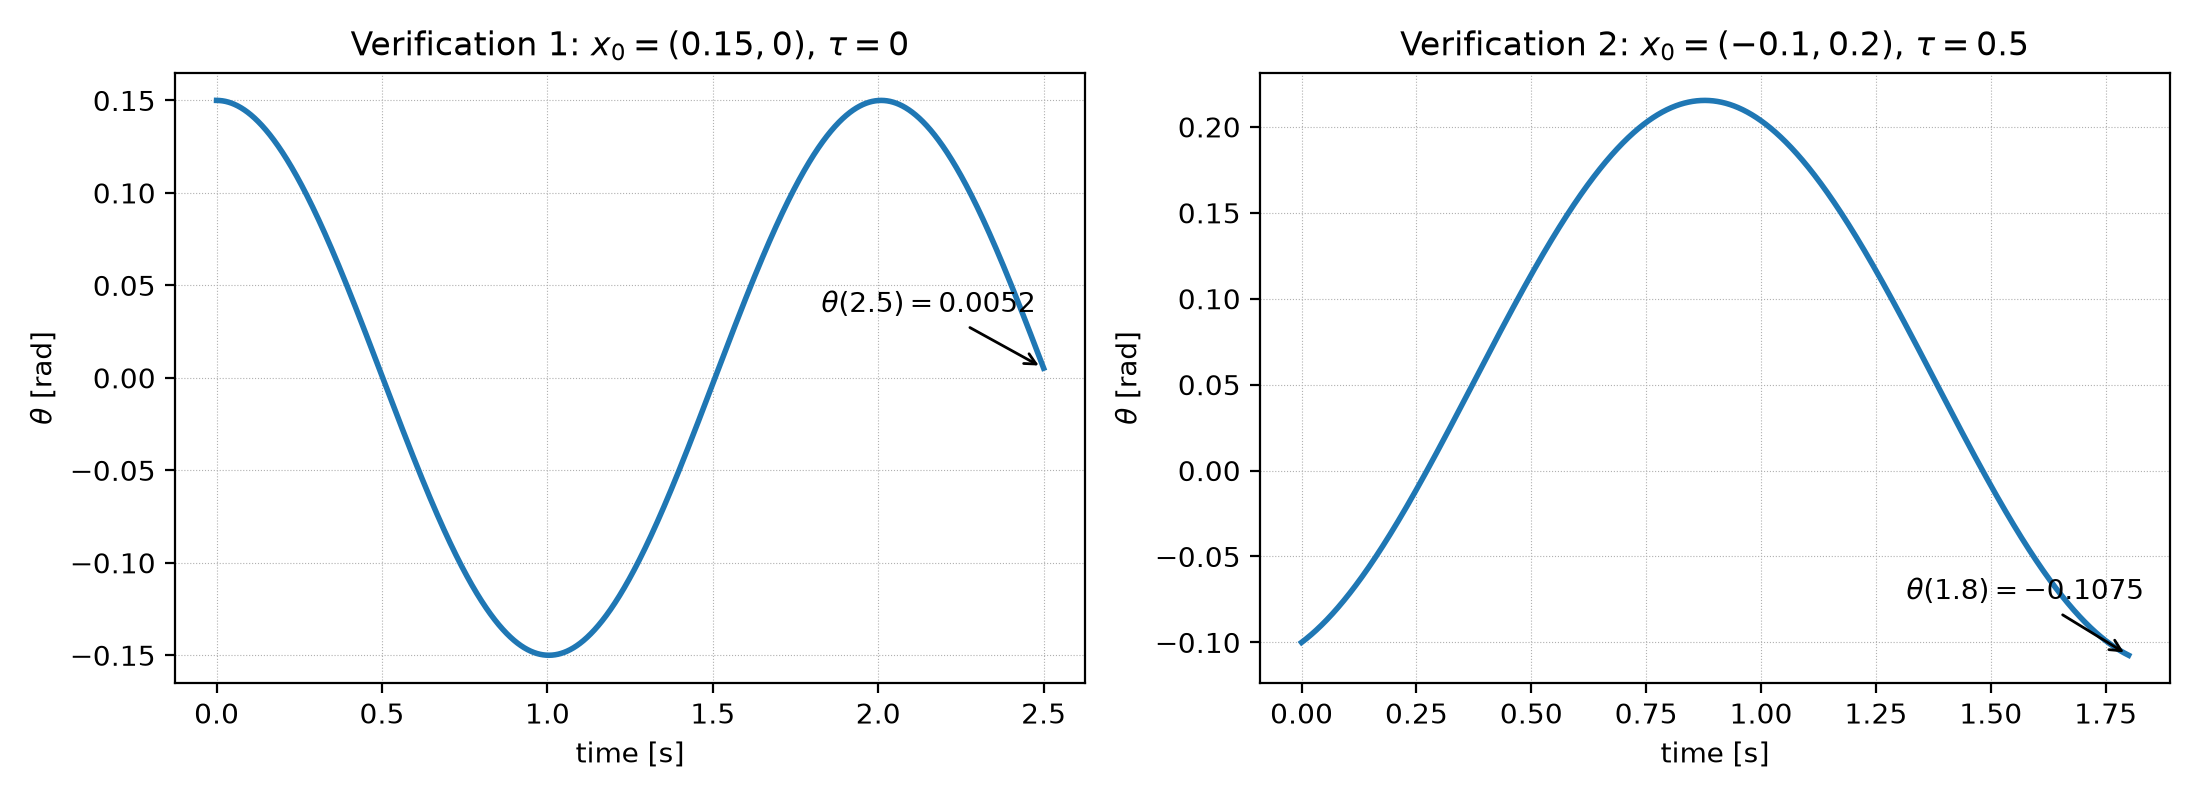
\includegraphics[width=0.9\textwidth]{ch1_pendulum.png}
\caption{Inverted-pendulum simulations for the two verification conditions.  The
final angles are 0.0052 and $-0.1074$~rad, matching the autograder.}
\end{figure}

\paragraph{Exercise 1.3: Physics Simulation and Robot Loading.}
The exercise loads a 7-DoF IIWA14 with \texttt{Parser} and
\texttt{MultibodyPlant}, welds the base, and adds a simple proportional
controller
\[
\tau=-K(q-q_d)
\]
with 14 inputs (seven positions and seven velocities) and seven torque outputs.
It then builds a table from an SDF string, generates letter assets with the
provided API, and assembles a full scene.  The visible autograders give
10/10 for the IIWA14 structure, 10/10 for the controller, 10/10 for the
full-system run, and 20/20 for the Gradescope verification, for a total of
50/50.  The verification target is
\[
q_{\rm final}=[0.0126,0.0081,-0.0573,-0.0244,-0.0001,0.0005,0.0000].
\]
The small residuals are due to gravity and joint damping; the P controller
does not compensate gravity.

\begin{figure}[htbp]
\centering
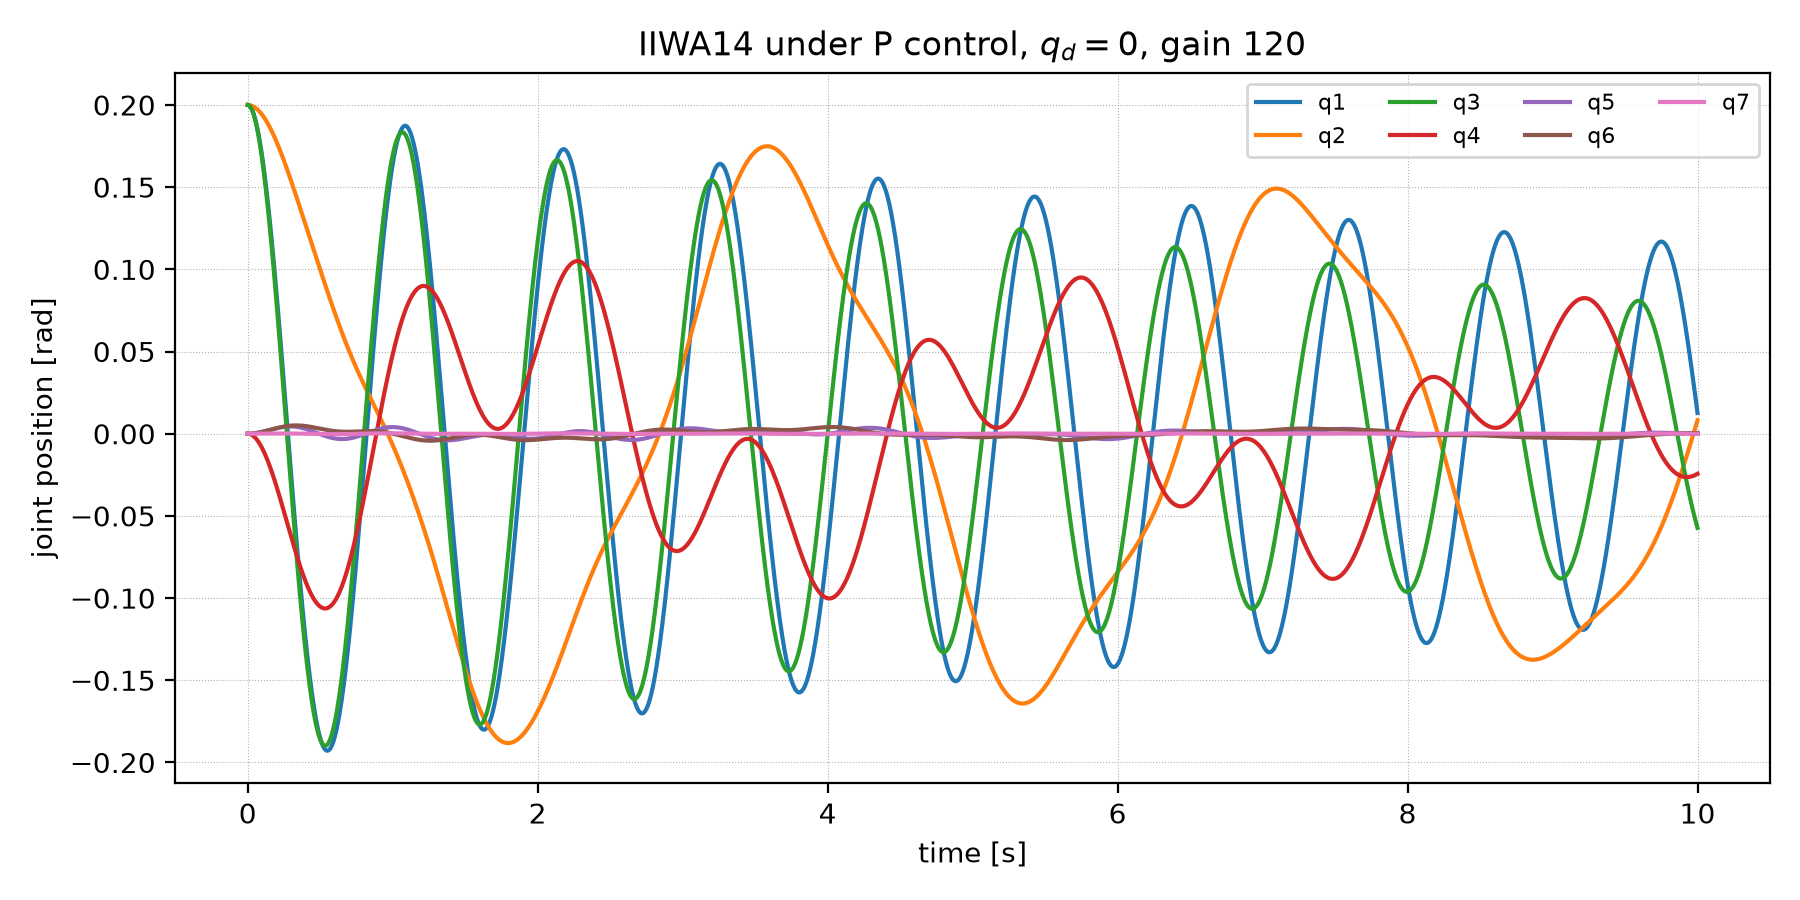
\includegraphics[width=0.9\textwidth]{ch1_iiwa.png}
\caption{Joint positions of the IIWA14 under the proportional controller.  The
residuals are below 0.06~rad; the P controller does not compensate gravity, so
a small steady-state offset remains.}
\end{figure}

\paragraph{Exercise 1.4: HardwareStation and Advanced Scenarios.}
This exercise replaces the manual wiring with a HardwareStation and a YAML
scenario.  The scenario contains two IIWA14 robots, a local table, three
letters and a free YCB object.  The station is added to a diagram and
simulated.  The autograders give 10/10 for the basic station, 10/10 for the
bimanual station, 15/15 for the full-system structure with eight model
instances, and 15/15 for the simulation run, for a total of 50/50.

\begin{lstlisting}[caption={Scenario directives for the bimanual station (abridged).}]
directives:
- add_model:
    name: iiwa_left
    file: package://drake_models/iiwa_description/urdf/iiwa14_primitive_collision.urdf
- add_weld:
    parent: world
    child: iiwa_left::iiwa_link_0
- add_model:
    name: iiwa_right
    file: package://drake_models/iiwa_description/urdf/iiwa14_primitive_collision.urdf
- add_weld:
    parent: world
    child: iiwa_right::iiwa_link_0
    X_PC:
        translation: [0.0, 1.0, 0.0]
- add_model:
    name: table
    file: file:///.../assets/table.sdf
- add_weld:
    parent: world
    child: table::table_link
    X_PC:
        translation: [0.5, 0.0, -0.05]
\end{lstlisting}

\section{Implementation notes}

I used the pinned \texttt{drake\_models} package for the IIWA14, the WSG
gripper and the YCB object.  The package was not present in the initial
environment; after it was placed in the local Drake cache, all notebooks ran
with \texttt{package://drake\_models}.  The teleoperation notebook was run with
\texttt{COLAB\_TESTING=1}; the 2D and 3D functions were simulated for 0.1~s.
The exercise notebooks use the official model and the local table/letter
assets, and the autograders give 70/70, 50/50 and 50/50.

\section{Discussion}

The teleoperation stack is deliberately local: differential IK tracks a pose,
but it does not avoid obstacles and it can get stuck near singularities.  The
System Diagrams example explains why the stack is organised as a diagram rather
than a single script; the HardwareStation scenario makes the same structure
declarative.  The P controller in Exercise~1.3 is also intentionally simple and
leaves a gravity-induced steady-state error.  For a real manipulation system,
the next steps would be a trajectory planner, a collision-aware IK or MPC
layer, and a gravity-compensating controller.

%=====================================================================
\chapter{Conclusions}
%=====================================================================

The four chapters share a common methodological pattern.  A model is written
in terms of state and inputs; a local linearisation is used to design a
controller; the nonlinear simulation is used to find the limits of the linear
design.  The limits appear in different forms in each chapter: saturation and
a finite basin for the acrobot and cart-pole; impact losses and a narrow basin
for the compass gait; energy conservation and partial stability for SLIP; and
contact planning for the legged robots.

The most consistent lesson is that underactuation and controllability answer
different questions.  The acrobot, cart-pole and quadrotor are all
underactuated, yet their linearisations are controllable.  What changes from
one system to the next is how much input authority is available in each
direction, and the singular values and nonlinear simulations show that this
difference can be the difference between a comfortable recovery and a
saturated failure.

A second observation is that LQR is a local tool.  The closed-loop eigenvalues
give local exponential stability, but they say little about the basin of
attraction or about what happens when the actuator saturates.  The acrobot and
cart-pole runs make this concrete: the same controller that recovers from a
small perturbation fails from a larger one or from a different direction.

The hybrid systems in Chapter~4 require a different object.  The limit cycle
and its return map replace the fixed point and the Jacobian.  Impact maps are
dissipative and can produce a stable gait, but the basin can be narrow; a
conservative model such as SLIP gives a one-dimensional apex map and only
partial stability.  The hopper controller is a good example of using the energy
balance directly instead of trying to track a trajectory.

Finally, planning and control are complementary.  The ZMP planner, the
LittleDog optimisation, MIQP and GCS all choose a contact sequence or a
reference trajectory; the feedback controller only tracks it.  The software
stack---Drake diagrams, URDF/SDF assets, differential IK and
HardwareStation---is what makes it possible to move between these levels
without rewriting the whole system.

\begin{thebibliography}{9}
\bibitem{tedrake-acrobot} R. Tedrake, \emph{Underactuated Robotics}, Chapter 3:
Acrobots, Cart-Poles, and Quadrotors. \url{https://underactuated.csail.mit.edu/acrobot.html}
\bibitem{tedrake-simplelegs} R. Tedrake, \emph{Underactuated Robotics}, Chapter 4:
Simple Models of Walking and Running. \url{https://underactuated.csail.mit.edu/simple_legs.html}
\bibitem{tedrake-humanoids} R. Tedrake, \emph{Underactuated Robotics}, Chapter 5:
Highly-articulated Legged Robots. \url{https://underactuated.csail.mit.edu/humanoids.html}
\bibitem{manipulation-intro} R. Tedrake, \emph{Robotic Manipulation}, Chapter 1:
Introduction. \url{https://manipulation.csail.mit.edu/intro.html}
\bibitem{drake-tutorials} Drake tutorials, including the dynamical systems and
authoring leaf systems tutorials, and the C++ doxygen page on spatial vectors.
\url{https://github.com/RobotLocomotion/drake/tree/master/tutorials},
\url{https://drake.mit.edu/doxygen_cxx/group__multibody__spatial__vectors.html}
\bibitem{lectures} Course lectures: 6.8210 Lecture 5 (Acrobots, cart-poles and
quadrotors), 6.832 Lecture 15 (Simple models of walking), 6.8210 Lecture 16
(Humanoid robots), and 6.4210 Lecture 1 (Introduction to manipulation).
\end{thebibliography}

%=====================================================================
\appendix
\chapter{Code and Reproduction}
\label{app:code}
%=====================================================================

The code is organised by chapter:

\begin{center}
\begin{tabular}{ll}
\toprule
Chapter & Main files \\
\midrule
Ch.~3 & \texttt{Ch-3/Ch3\_Assignment\_Report/code/} \\
Ch.~4 & \texttt{Ch-4/Ch4\_Assignment\_Report/code/} \\
Ch.~5 & \texttt{Ch-5/Ch5\_Assignment\_Report/code/} \\
Ch.~1 & \texttt{Ch-1/Ch1\_Assignment\_Report/code/} \\
\bottomrule
\end{tabular}
\end{center}

The notebooks can be executed headlessly with
\begin{lstlisting}[language=bash]
COLAB_TESTING=1 /Users/leo/venvs/drake/bin/jupyter nbconvert \
  --to notebook --execute --inplace --ExecutePreprocessor.timeout=300 \
  <notebook>.ipynb
\end{lstlisting}
\begin{sloppypar}
and the reports are compiled with \texttt{pdflatex} run twice.  The combined
code is in \texttt{Assignment\_1\_Code.zip}.
\end{sloppypar}

\section{Selected code}

\paragraph{Cart-pole dynamics and LQR.}
\begin{lstlisting}[language=Python]
def f(x, u):
    c, s = np.cos(x[1]), np.sin(x[1])
    g = 9.81
    return np.array([
        x[2], x[3],
        (u[0] + s * (x[3]**2 + g * c)) / (1 + s**2),
        (-u[0] * c - x[3]**2 * c * s - 2 * g * s) / (1 + s**2)])
\end{lstlisting}

\paragraph{Double-pendulum URDF.}
\begin{lstlisting}[language=XML]
<link name="pendulum1">
  <inertial>
    <origin xyz="0 0 1" />
    <mass value="1" />
    <inertia ixx="0" ixy="0" ixz="0" iyy="0" iyz="0" izz="0" />
  </inertial>
</link>
<joint name="theta1" type="continuous">
  <parent link="pendulum0" />
  <child link="pendulum1" />
  <origin xyz="0 0 -1" />
  <axis xyz="0 -1 0" />
</joint>
\end{lstlisting}

\paragraph{Hopper controller.}
\begin{lstlisting}[language=Python]
def get_delta_bar(self, state):
    k, mb, ml, g = self.hopper_parameters
    zb = state[0]
    return (0.5 * zb + mb * g / k
            - ((mb + ml) ** 2) * g * self.h / (k * mb * zb))
\end{lstlisting}

\paragraph{Cart-pole LQR wiring (Chapter 3).}
\begin{lstlisting}[language=Python]
def cartpole_balancing(cartpole_urdf, x_star, Q, R):
    builder = DiagramBuilder()
    plant, scene_graph = AddMultibodyPlantSceneGraph(builder, time_step=0.0)
    Parser(plant).AddModelsFromString(cartpole_urdf, "urdf")
    plant.Finalize()
    plant.set_name("cartpole")

    context = plant.CreateDefaultContext()
    context.get_mutable_continuous_state_vector().SetFromVector(x_star)
    plant.get_actuation_input_port().FixValue(context, [0])
    input_i = plant.get_actuation_input_port().get_index()

    lqr = LinearQuadraticRegulator(
        plant, context, Q, R, input_port_index=input_i)
    lqr = builder.AddSystem(lqr)
    builder.Connect(plant.get_state_output_port(), lqr.get_input_port(0))
    builder.Connect(lqr.get_output_port(0),
                    plant.get_actuation_input_port())
    return builder.Build()
\end{lstlisting}

\paragraph{Inverted pendulum system (Chapter 1).}
\begin{lstlisting}[language=Python]
class InvertedPendulum(LeafSystem):
    def __init__(self, mass=1.0, length=1.0, gravity=9.81):
        LeafSystem.__init__(self)
        self.mass, self.length, self.gravity = mass, length, gravity
        self.DeclareContinuousState(2)
        self.torque_port = self.DeclareVectorInputPort("torque", 1)
        self.DeclareVectorOutputPort("theta", 1, self.OutputTheta)

    def DoCalcTimeDerivatives(self, context, derivatives):
        x = context.get_continuous_state_vector()
        theta, theta_dot = x[0], x[1]
        torque = self.torque_port.Eval(context)[0]
        theta_ddot = -self.gravity * np.sin(theta) + torque / (
            self.mass * self.length**2)
        derivatives.get_mutable_vector().SetFromVector(
            [theta_dot, theta_ddot])

    def OutputTheta(self, context, output):
        output.SetFromVector([context.get_continuous_state_vector()[0]])
\end{lstlisting}

\paragraph{Hopper controller logic (Chapter 4).}
\begin{lstlisting}[language=Python]
def is_bottom_or_apex(self, state):
    if np.any(np.isnan(self.last_state)):
        return None
    zb, l, zb_dot, l_dot = state
    last_zb_dot = self.last_state[2]
    if last_zb_dot <= 0.0 and zb_dot > 0.0:
        return "bottom" if zb < 0.0 else "apex"
    if last_zb_dot >= 0.0 and zb_dot < 0.0:
        return "apex" if zb > 0.0 else "bottom"
    return None

def DoCalcVectorOutput(self, context, delta):
    state = self.get_input_port(0).Eval(context)
    event = self.is_bottom_or_apex(state)
    if event == "bottom":
        delta.SetFromVector([max(self.get_delta_bar(state), 0.0)])
    elif event == "apex":
        delta.SetFromVector([0.0])
    else:
        delta.SetFromVector([self.last_delta])
    self.last_delta = delta[0]
    self.last_state = np.array(state)
\end{lstlisting}

\paragraph{HardwareStation scenario.}
The scenario in Exercise~1.4 uses \texttt{add\_model}, \texttt{add\_weld} and
\texttt{default\_free\_body\_pose} directives; the local table and letters are
referenced by absolute \texttt{file://} URIs, while the robots and the YCB
object use \texttt{package://drake\_models}.

\end{document}
